\documentclass[12pt,letterpaper]{article}

% ---- Encoding & fonts ----------------------------------------------------
\usepackage[utf8]{inputenc}
\usepackage[T1]{fontenc}
\usepackage{mathptmx}                   % Times-like body + math (APA-friendly)
\usepackage[scaled=0.92]{helvet}        % matching sans
\usepackage{courier}
\usepackage{microtype}

% ---- Layout --------------------------------------------------------------
\usepackage[letterpaper, margin=0.8in]{geometry}
\usepackage{setspace}
\doublespacing
\usepackage{parskip}
\usepackage{titlesec}
\titleformat{\section}{\normalfont\large\bfseries}{\thesection.}{0.6em}{}
\titleformat{\subsection}{\normalfont\normalsize\bfseries}{\thesubsection}{0.6em}{}
\titlespacing*{\section}{0pt}{1.2ex plus 0.4ex}{0.6ex}
\titlespacing*{\subsection}{0pt}{1.0ex plus 0.4ex}{0.4ex}

% ---- Headers / page numbering -------------------------------------------
\usepackage{fancyhdr}
\pagestyle{fancy}\fancyhf{}
\fancyfoot[C]{\thepage}
\fancyhead[L]{}
\renewcommand{\headrulewidth}{0pt}

% ---- Math ----------------------------------------------------------------
\usepackage{amsmath,amssymb,amsfonts}
\usepackage{bm}

% ---- Tables --------------------------------------------------------------
\usepackage{booktabs}
\usepackage{array}
\usepackage{tabularx}
\usepackage{longtable}
\usepackage{multirow}
\usepackage{ragged2e}
\renewcommand{\arraystretch}{0.66}
\newcolumntype{L}[1]{>{\RaggedRight\arraybackslash}p{#1}}
\newcolumntype{C}[1]{>{\centering\arraybackslash}p{#1}}
\newcolumntype{R}[1]{>{\RaggedLeft\arraybackslash}p{#1}}

% ---- Figures -------------------------------------------------------------
\usepackage{graphicx}
\usepackage{float}
\usepackage[font=small,labelfont=bf,labelsep=period]{caption}
\usepackage{subcaption}
\graphicspath{{figure/}{figures/}{outputs/figures/}{analysis/outputs/figures/}}

% ---- Citations -----------------------------------------------------------
\usepackage[round, authoryear]{natbib}
\bibpunct{(}{)}{;}{a}{,}{,}

% ---- Lists ---------------------------------------------------------------
\usepackage{enumitem}
\setlist[itemize]{leftmargin=*, itemsep=2pt, topsep=3pt}
\setlist[enumerate]{leftmargin=*, itemsep=2pt, topsep=3pt}

% ---- Color & links -------------------------------------------------------
\usepackage{xcolor}
\usepackage[colorlinks=true,linkcolor= blue!65!black
,citecolor=blue!50!black ,
            urlcolor=blue!50!black]{hyperref}

% =========================================================================

\title{
    \vspace{4cm}
    \textbf{Measuring Regional Disparities in China's \\Digital Economy Development:\\
    A Multivariate Analysis \\ Using PCA and Factorial MANOVA, 2013--2022}
}

\author{
    Airui Meng\\[6pt]
    Department of Human Development, Teachers College, Columbia University\\
    HUDM 6122: Multivariate Analysis I
}

\date{}

% =========================================================================
\begin{document}

\vspace{4cm}
\maketitle
\thispagestyle{plain}

\newpage
% ============================ ABSTRACT ===================================
\begin{center}
\begin{minipage}{0.92\textwidth}
\setstretch{1.5}
\centering{\large\textbf{Abstract}} \,

\vspace{1cm}

The rapid expansion of China's digital economy has transformed regional development patterns, yet whether this transformation has narrowed or widened existing geographic disparities remains an open empirical question. Using a panel of 31 mainland Chinese provinces over 2013--2022 and a 22-indicator system organized along three dimensions (digital infrastructure, digital industry, digital environment), this study (a) constructs a composite Digital Economy Development Index (DEDI) via principal component analysis (PCA) and (b) tests for regional and temporal differences via a factorial MANOVA on retained component scores. Four orthogonal components (cumulative variance $85.8\%$) are retained
and interpreted as {Industry/Innovation Scale}, {Per-capita Penetration},
{Infrastructure Connectivity}, and {Enterprise Digitalization}. The
$4 \times 2$ factorial design (Region $\times$ Period) yields large multivariate main
effects of region (Pillai's $V=0.754$, $\eta^{2}=0.25$) and period
($V=0.719$, $\eta^{2}=0.72$) but a non-significant interaction
($V=0.021$, $p=.892$), indicating that while every region advanced substantially
between the two five-year periods, the relative rank ordering of regions has remained
essentially time-invariant. Sensitivity analyses on three single-year cross-sections
and on outlier-removed subsamples confirm robustness.

\vspace{0.5em}
\noindent\textbf{Keywords.} \, digital economy measurement; principal component analysis (PCA);
factorial MANOVA; Pillai's trace; regional disparity; China provincial panel.
\end{minipage}
\end{center}

\vspace{1em}
% =========================================================================
\newpage
\section{Introduction}
% =========================================================================

The digital economy --- defined by the International Telecommunication Union as ``all economic activities facilitated by digital computing technologies'' --- has emerged as a principal driver of growth and structural transformation in China.  By 2022 the digital economy accounted for a substantial share of national GDP, but its diffusion has been highly uneven across the country, exacerbating long-standing east--west and coastal--interior disparities \citep{he2023}.  A central concern for policymakers is therefore not merely the average level of digital development, but the {multidimensional} shape of regional differences: are gaps closing on infrastructure but widening on per-capita penetration?  Has the relative ordering of provinces changed
across time?

Existing work on Chinese digital-economy measurement is dominated by composite indices built from entropy-weighting, TOPSIS, or principal-component aggregation \citep{bai2024}.  These studies almost universally report descriptive heat maps and ranks, but rarely apply formal multivariate inference to test whether regional differences are statistically significant once the multidimensional nature of the construct is acknowledged.  Two methodological gaps are particularly salient.  First, regression and ANOVA-based comparisons examine one
dependent variable at a time, ignoring the substantial within-construct
correlations among indicators that motivate the use of an index in the first place.  Second, when researchers do select ``representative'' indicators from the loadings of a prior PCA and submit them to MANOVA, the resulting analysis is contaminated by data-driven variable selection on the very same variance structure that drives the inference.

This study addresses both gaps in a methodologically clean way.  We first reduce 22 third-level indicators to four orthogonal principal components and then use the resulting {component scores}, rather than hand-picked indicators, as the multivariate dependent variables in a $4 \times 2$ factorial MANOVA. The two factors are official economic region (East, Central, West, Northeast) and time period (Early 2013--2017 vs. Late 2018--2022).  This approach \citep{tabachnick2019} guarantees that the dependent variables are mutually orthogonal --- automatically satisfying the multicollinearity assumption of MANOVA --- while preserving all the variance information of the original indicator system.

The study is guided by four research questions.

\textbf{RQ1}. What is the underlying multidimensional structure of provincial digital-economy development between 2013 and 2022?

\textbf{RQ2}. Do the four official economic regions of China differ simultaneously on multiple dimensions of digital-economy development?

\textbf{RQ3}. Has the regional structure of the digital economy shifted between the early period (2013--2017) and the late period (2018--2022),i.e.~is there a Region $\times$ Period interaction?

\textbf{RQ4}. Are the answers to RQ2--RQ3 robust to (i)~the choice of reference year, (ii)~the temporal stability of the underlying components, and (iii)~the presence of multivariate outliers?


The remainder of the paper is organised as follows.  Section~\ref{sec:method}
develops the econometric framework.  Section~\ref{sec:data} describes the data
and indicator system.  Section~\ref{sec:results} presents empirical results.
Section~\ref{sec:discuss} discusses implications, limitations, and concludes.

% =========================================================================
\section{Methodology}\label{sec:method}
% =========================================================================

\subsection{Indicator system and pre-processing}

Following the framework of \citet{he2023}, the 22 third-level indicators
$X_{1},\dots,X_{22}$ are nested under three first-level dimensions: digital
infrastructure (six indicators), digital industry (five indicators), and
digital environment (eleven indicators); see Table~\ref{tab:indicators} in
Section~\ref{sec:data}.  Twelve indicators with absolute sample skewness above
$1.5$ are log-transformed to attenuate the influence of provincial outliers
(notably Beijing, Shanghai, Guangdong) on the variance structure.  All
indicators are then $z$-score standardised so that the resulting
$310 \times 22$ matrix $\bm{Z}$ has columns of zero mean and unit variance.

\subsection{Principal component analysis}

Letting $\bm{R}$ denote the sample correlation matrix of $\bm{Z}$, PCA
decomposes
\begin{equation}
  \bm{R}\, \bm{a}_{j} \;=\; \lambda_{j}\,\bm{a}_{j},
  \qquad j = 1,\dots,p,
  \label{eq:eig}
\end{equation}
where $\lambda_{1}\geq\lambda_{2}\geq\cdots\geq\lambda_{p}\geq 0$ are the
eigenvalues and $\bm{a}_{j}$ the eigenvectors.  The factor model is
\begin{equation}
  \bm{Z} \;=\; \bm{F}\,\bm{A}^{\!\top} \,+\, \bm{E},
  \qquad \bm{F} = \bm{Z}\bm{A}(\bm{A}^{\!\top}\bm{A})^{-1},
  \label{eq:pca}
\end{equation}
where $\bm{F}$ is the $310\times k$ matrix of component scores and $\bm{A}$ the
$22\times k$ matrix of loadings for the $k$ retained components.  Sampling
adequacy is assessed by the Kaiser--Meyer--Olkin (KMO) measure
\citep{kaiser1974} and Bartlett's test of sphericity.  The number of components
is chosen as $k = \max\!\bigl(k_{\text{Kaiser}},\,k_{80\%}\bigr)$, where
$k_{\text{Kaiser}}$ is the number of $\lambda_{j}\geq 1$ and $k_{80\%}$ is the
smallest $k$ such that $\sum_{j=1}^{k}\lambda_{j}/p \geq 0.80$.  A Varimax
rotation is applied to the retained loadings to aid substantive interpretation.

\subsection{Composite Digital Economy Development Index (DEDI)}

A scalar summary index is constructed as the variance-share-weighted, sign-aligned
sum of the retained component scores, rescaled to $[0,100]$:
\begin{equation}
  \text{DEDI}_{it} \;=\; 100 \cdot
  \frac{ \widetilde{F}_{it} - \min \widetilde{F}}{\max \widetilde{F} - \min \widetilde{F}},
  \qquad
  \widetilde{F}_{it} \;=\; \sum_{j=1}^{k} w_{j}\, s_{j}\, F_{j,it},
  \qquad
  w_{j} \;=\; \frac{\lambda_{j}}{\sum_{l=1}^{k}\lambda_{l}},
  \label{eq:dedi}
\end{equation}
where $s_{j}\in\{-1,+1\}$ flips any component whose summed correlation with the
raw indicators is negative so that ``higher = more digital'' for every
component.  DEDI is used only for descriptive ranking; the inferential analysis
operates directly on the four orthogonal scores $F_{1},\dots,F_{4}$.

\subsection{Factorial MANOVA}

Let $\bm{Y}_{ij\ell} = (F_{1,ij\ell}, \dots, F_{k,ij\ell})^{\!\top}$ be the
vector of component scores for the $\ell$-th observation in region $i$ and
period $j$.  The two-way fixed-effects multivariate model is
\begin{equation}
  \bm{Y}_{ij\ell} \;=\; \bm{\mu} \,+\, \bm{\alpha}_{i} \,+\, \bm{\beta}_{j}
  \,+\, (\bm{\alpha\beta})_{ij} \,+\, \bm{\varepsilon}_{ij\ell},
  \qquad
  \bm{\varepsilon}_{ij\ell} \overset{iid}{\sim} \mathcal{N}_{k}(\bm{0},\bm{\Sigma}),
  \label{eq:manova}
\end{equation}
$i = 1,\dots,4$ regions, $j=1,2$ periods, and $\ell = 1,\dots,n_{ij}$.
Multivariate hypotheses are tested using Pillai's trace as the primary statistic,
\begin{equation}
  V \;=\; \mathrm{tr}\!\left[\bm{H}\,(\bm{H}+\bm{E})^{-1}\right]
        \;=\; \sum_{r=1}^{s}\frac{\theta_{r}}{1+\theta_{r}},
  \label{eq:pillai}
\end{equation}
where $\bm{H}$ and $\bm{E}$ are the hypothesis and error sum-of-squares-and-products
matrices, $\theta_{r}$ are the non-zero eigenvalues of $\bm{H}\bm{E}^{-1}$, and
$s = \min(\nu_{H},k)$.  Pillai's $V$ is preferred because it is the
{most robust} of the four standard MANOVA criteria when covariance
homogeneity is violated \citep{pillai1955,tabachnick2019}.  Wilks' $\Lambda$,
Hotelling--Lawley's $T^{2}$, and Roy's largest-root statistic are reported for
transparency.  Multivariate effect sizes are summarised by partial $\eta^{2}$.

\subsection{Assumption diagnostics and post hoc procedures}

Multivariate normality is assessed by Mardia's tests of multivariate skewness
and kurtosis \citep{mardia1970} both overall and within each of the eight
$\text{region}\times\text{period}$ cells.  Covariance homogeneity is examined
with Box's $M$ test \citep{box1949}; per-DV variance homogeneity with Levene's
test; multivariate outliers via Mahalanobis distances against the
$\chi^{2}_{.999,k}$ quantile.  A significant multivariate test is decomposed by
univariate Type-II ANOVAs on each component, with pairwise region contrasts
estimated by the Games--Howell procedure \citep{games1976}, which does not
assume equal variances or equal cell sizes.

% =========================================================================
\section{Data and Variables}\label{sec:data}
% =========================================================================

\subsection{Sources and sample}

Data are drawn from the {China Statistical Yearbook} \textit{(\href{https://www.stats.gov.cn/english/Statisticaldata/yearbook/}{URL})}, the
{Statistical Yearbook of China's Tertiary Industry} \textit{(\href{http://www.tjcn.org/e/search/result/?searchid=1257}{URL})}, the {China Science and Technology Statistical Yearbook} \textit{(\href{https://www.tjnj.net/yearbookbyarea/china}{URL})}, and the Digital Inclusive Finance Index published by the Digital Finance Research Center of Peking University \textit{(\href{https://idf.pku.edu.cn/zsbz/bjdxszphjrzs/index.htm}{URL})}, all for fiscal years 2013--2022. The unit of observation is the province--year; the panel covers all $31$ mainland provinces (Hong Kong, Macao, and Taiwan are excluded), giving
$N = 310$ observations.  Panel structure is summarised in Table~\ref{tab:sample}.

\begin{table}[H]
\centering
\caption{Sample structure.}\label{tab:sample}
\begin{tabular}{l l}
\toprule
\textbf{Item} & \textbf{Value} \\
\midrule
Provinces            & 31 (mainland China; HK / Macao / Taiwan excluded) \\
Period               & 2013--2022 (10 years) \\
Observations         & 310 (province--year) \\
Indicators           & 22 third-level under 3 first-level dimensions \\
Regions ($g=4$)      & East 10 \quad Central 6 \quad West 12 \quad Northeast 3 \\
Period split         & Early 2013--2017 ($n=155$) \quad Late 2018--2022 ($n=155$)\\
\bottomrule
\end{tabular}
\end{table}

\subsection{Indicator system}

The 22 third-level indicators are organised into seven second-level and three
first-level dimensions following \citet{he2023}.  Table~\ref{tab:indicators}
provides the full hierarchy with the symbol used throughout the paper.

\begin{table}[H]
\centering
\caption{Hierarchical indicator system (3 first-level, 7 second-level, 22 third-level).}
\label{tab:indicators}
\small
\begin{tabularx}{\textwidth}{@{} L{0.2\textwidth} L{0.22\textwidth} L{0.51\textwidth} @{}}
\toprule
\textbf{First-level} & \textbf{Second-level} & \textbf{Third-level indicator}\\
\midrule
\multirow{2}{=}{Digital Infrastructure}
  & Hardware  & $x_1$ Optical cable;  $x_2$ broadband ports; \par  $x_3$ mobile base stations\\
  & Software  &  $x_4$ domain names;  $x_5$ IPv4 addresses;  $x_6$ websites\\
\midrule
\multirow{2}{=}{Digital Industry Development}
  & Industrialisation & $x_7$ software business revenue; $x_8$ telecom revenue\\
  & Industrial digitalisation & $x_9$ websites/100 enterprises; $x_{10}$ \% e-commerce firms; \par $x_{11}$ e-commerce sales\\
\midrule
\multirow{3}{=}{Digital Environment}
  & Application & $x_{12}$ computers/100 people; $x_{13}$ mobile internet users; $x_{14}$ mobile phone subscribers; $x_{15}$ digital TV; $x_{16}$ digital inclusive finance index; $x_{17}$ digital--real integration\\
  & Talent      & $x_{18}$ \% IT employment; $x_{19}$ bachelor's graduates\\
  & Innovation  & $x_{20}$ R\&D personnel (FTE); $x_{21}$ R\&D institutions; \par $x_{22}$ regional patent grants\\
\bottomrule
\end{tabularx}
\end{table}

\subsection{Pre-processing footprint}

Linear interpolation in the time dimension was applied to fill missing cells in
the raw yearbooks.  Of the $22\times 310 = 6{,}820$ panel cells, only three
indicators required imputation: $x_{5}$ IPv4 addresses ($20.3\%$ of cells),
$x_{13}$ mobile internet users ($8.4\%$), and $x_{21}$ R\&D institutions
($0.3\%$).  All other 19 indicators are observed in full.

\subsection{Regional classification}

The four official economic regions follow the National Bureau of Statistics
classification.  We key the assignment off the provincial GB-2260 administrative
codes (e.g.~$110000=$ Beijing $\to$ East) to avoid encoding ambiguity:
the East comprises Beijing, Tianjin, Hebei, Shanghai, Jiangsu, Zhejiang, Fujian,
Shandong, Guangdong, Hainan; the Central, Shanxi, Anhui, Jiangxi, Henan, Hubei,
Hunan; the West, twelve provinces from Inner Mongolia to Xinjiang; and the
Northeast, Liaoning, Jilin, Heilongjiang.

% =========================================================================
\section{Empirical Results}\label{sec:results}
% =========================================================================

\subsection{Sampling adequacy and component retention}

The data are highly suitable for PCA: the overall KMO measure of sampling
adequacy is $0.904$ (``meritorious'' per the conventional thresholds of
\citealp{kaiser1974}), with only $x_{9}$ falling below $0.7$.  Bartlett's test
of sphericity strongly rejects the identity hypothesis,
$\chi^{2}(231) = 11{,}553.82$, $p<.001$, supporting factorability.

Eigenvalue decomposition (Eq.~\ref{eq:eig}) yields four components with
$\lambda_{j}\geq 1$ and three components reaching cumulative variance of $80.6\%$
(Table~\ref{tab:eigen}).  Applying the conservative
$k = \max(k_{\text{Kaiser}}, k_{80\%}) = 4$ rule retains \textbf{four}
components explaining $85.8\%$ of total variance.  The scree plot
(Figure~\ref{fig:scree}) corroborates the elbow between PC4 and PC5.

\begin{table}[H]
\centering
\caption{Eigenvalues and variance explained (first five PCs).}\label{tab:eigen}
\begin{tabular}{c r r r}
\toprule
\textbf{PC} & \textbf{Eigenvalue} & \textbf{Variance \%} & \textbf{Cumulative \%}\\
\midrule
1 & 12.98 & 59.0 & 59.0 \\
2 &  2.90 & 13.2 & 72.2 \\
3 &  1.84 &  8.4 & 80.6 \\
4 &  1.16 &  5.3 & \textbf{85.8} \\
5 &  0.66 &  3.0 & 88.8 \\
\bottomrule
\end{tabular}
\end{table}

\begin{figure}[H]
\centering
\begin{subfigure}[t]{0.48\textwidth}
  \centering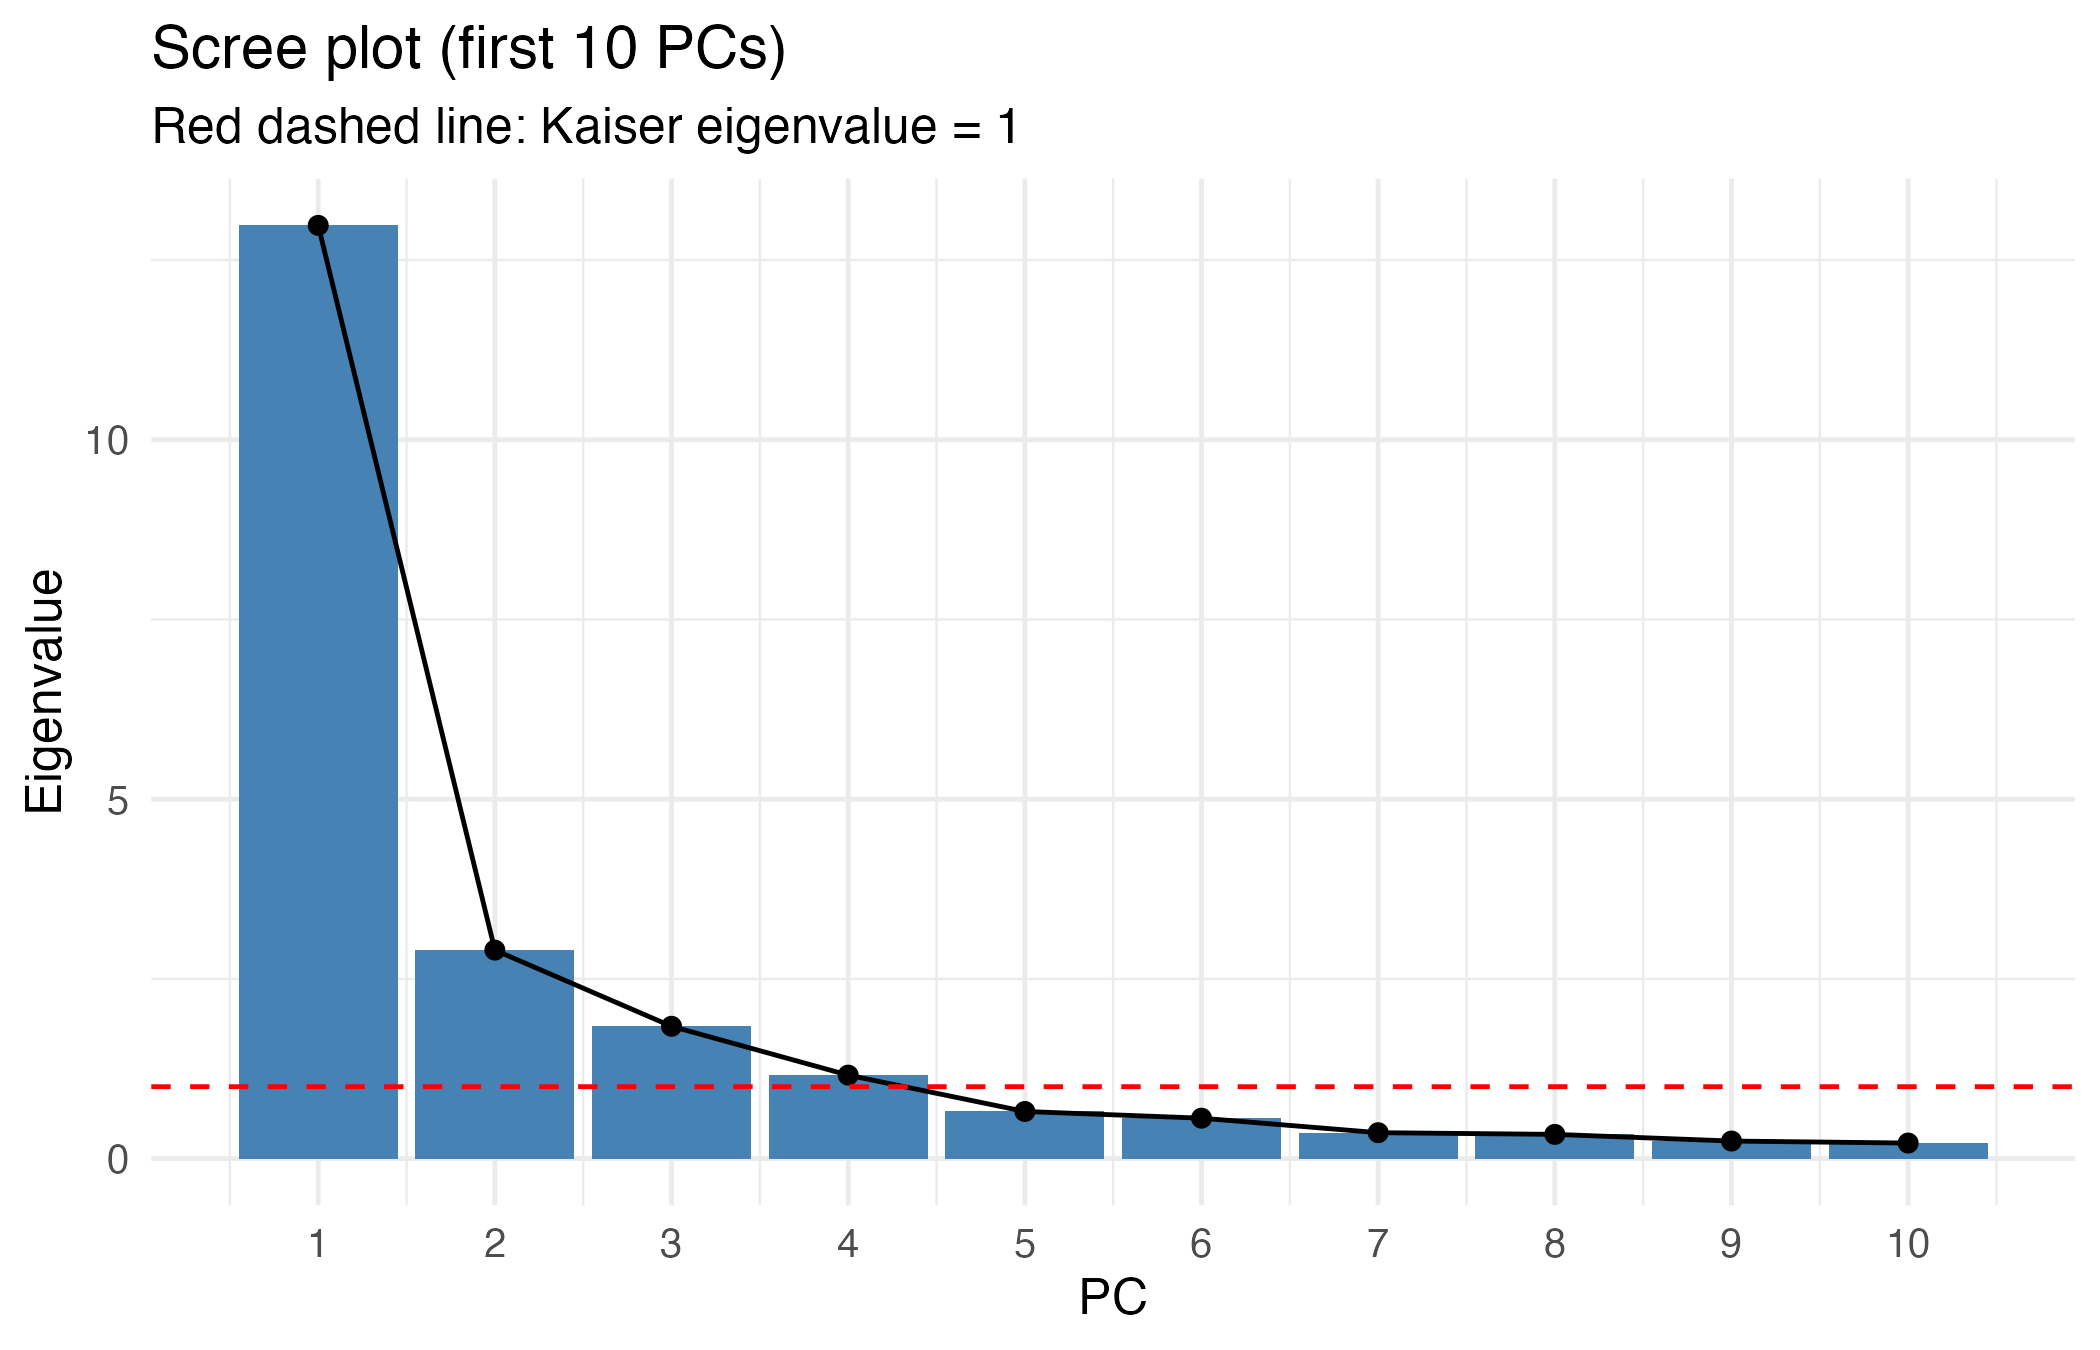
\includegraphics[width=\linewidth]{02_scree.png}
  \caption{Scree plot. Red dashed line: Kaiser eigenvalue $=1$.}
\end{subfigure}\hfill
\begin{subfigure}[t]{0.48\textwidth}
  \centering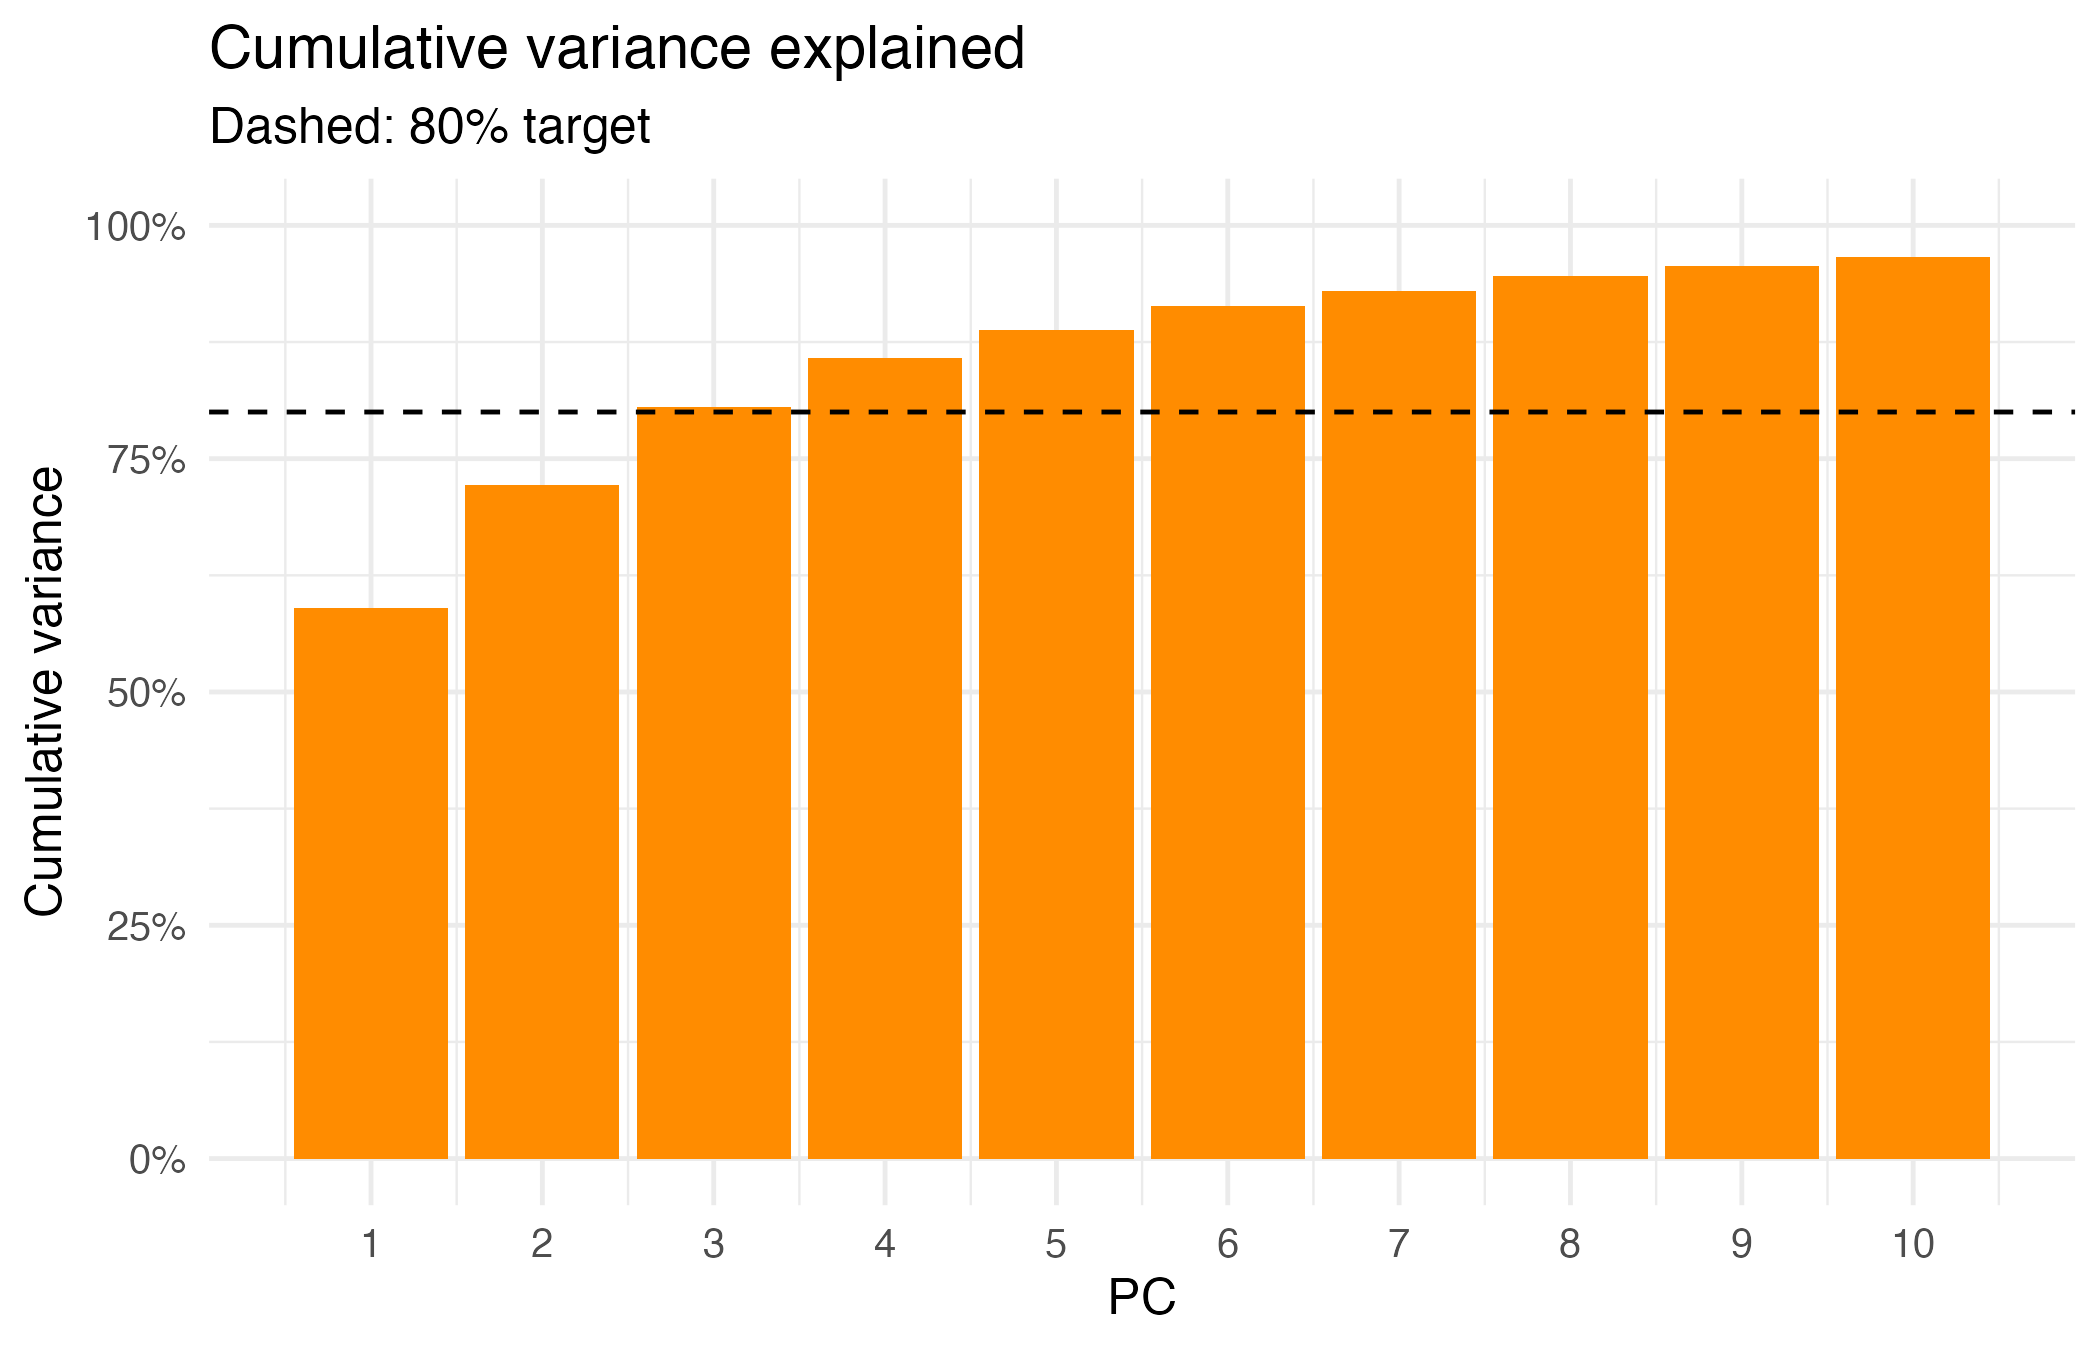
\includegraphics[width=\linewidth]{02_cumvar.png}
  \caption{Cumulative variance explained.  Dashed line: $80\%$ target.}
\end{subfigure}
\caption{PCA retention diagnostics.}\label{fig:scree}
\end{figure}

\subsection{Component interpretation}

After Varimax rotation, the four components have a clean simple-structure
pattern (Figure~\ref{fig:loadings}).  RC1 loads heavily on indicators of
{absolute} digital scale (R\&D personnel, patents, e-commerce sales,
software revenue, IPv4 addresses); we label it
\textbf{Industry / Innovation Scale}.  RC2 loads negatively (and after sign
flipping, positively) on {per-capita / penetration} indicators ($\%$
e-commerce firms, computers per 100 people, digital inclusive finance, $\%$
IT employment); we label it \textbf{Per-capita Penetration}.  RC3 loads on
infrastructure-stock indicators (optical cable, broadband ports, base stations,
mobile users, digital TV) and is labelled \textbf{Infrastructure Connectivity}.
RC4 is dominated by $x_9$ (websites per 100 enterprises) and is labelled
\textbf{Enterprise Digitalization Intensity}.

\begin{figure}[H]
\centering
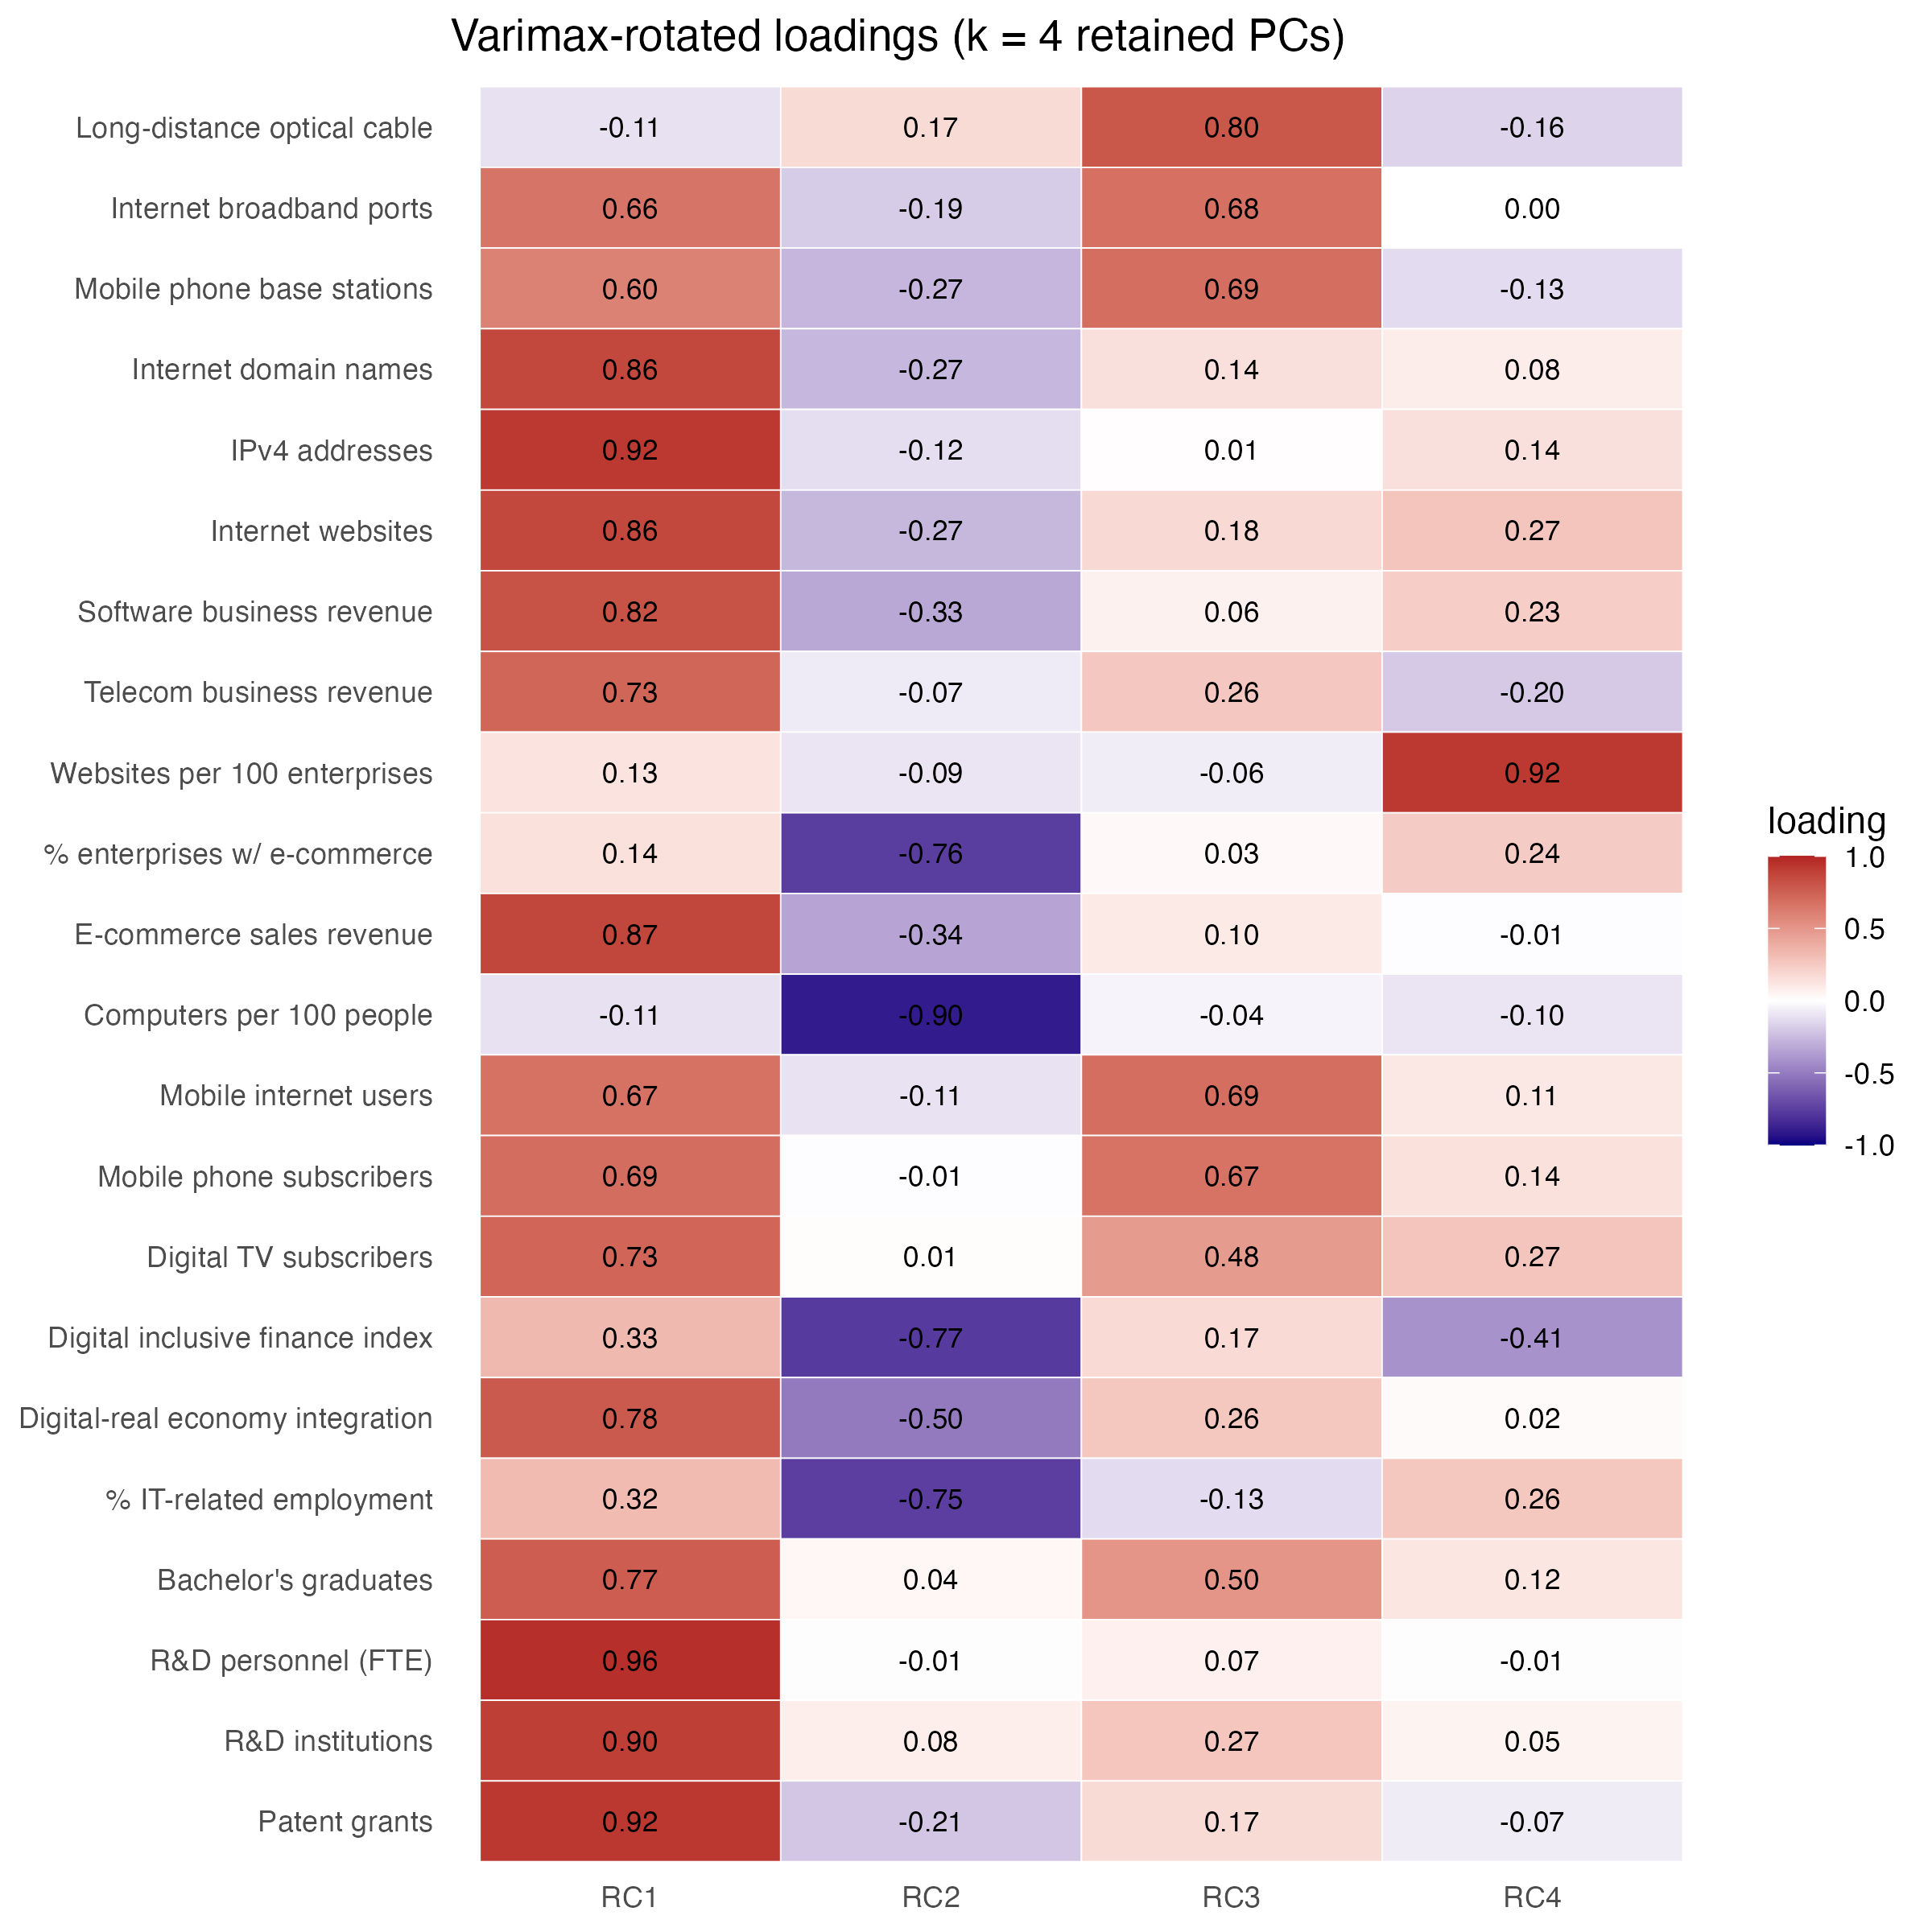
\includegraphics[width=0.78\textwidth]{02_loadings_heatmap.png}
\caption{Varimax-rotated loadings of the 22 indicators on the four retained PCs.}
\label{fig:loadings}
\end{figure}

\subsection{Composite DEDI: spatial and temporal patterns}

The variance-share weights (Eq.~\ref{eq:dedi}) are
$w = (0.687,\,0.154,\,0.097,\,0.062)$ and the sign-flip vector is
$s=(+1,-1,+1,+1)$.  In the 2019 cross-section, the highest DEDI scores belong
to Guangdong ($95.0$), Jiangsu ($80.7$), Zhejiang ($76.5$), Shandong ($76.1$),
and Beijing ($74.8$); the lowest are Tibet ($21.2$), Qinghai ($24.6$), and
Ningxia ($28.2$).  Notably, Sichuan ranks $6$th --- the only Western province in
the top ten --- while Hainan ranks $27$th despite belonging to the East,
illustrating that regional means hide substantial within-region heterogeneity.

Region-mean DEDI rises in every region between the two periods, but the
{rate} of progress is uneven (Table~\ref{tab:cellmeans}): Central provinces
post the largest gain ($+14.2$ DEDI points), narrowly ahead of the East
($+12.2$), with the Northeast lagging clearly ($+8.1$).  Inter-provincial
dispersion increases in absolute terms (the standard deviation of DEDI rises
from $15.4$ in 2013 to $18.0$ in 2022) yet shrinks in relative terms
(the coefficient of variation falls from $0.43$ to $0.32$) ---
$\sigma$-divergence with $\beta$-convergence (Figure~\ref{fig:dedi-time}).

\begin{table}[H]
\centering
\caption{Region $\times$ period mean DEDI (rescaled $0$--$100$).}
\label{tab:cellmeans}
\begin{tabular}{l r r r}
\toprule
\textbf{Region} & \textbf{Early (2013--17)} & \textbf{Late (2018--22)} & $\bm{\Delta}$\\
\midrule
East      & 56.12 & 68.34 & $+12.22$\\
Central   & 44.13 & 58.31 & $+14.18$\\
West      & 31.62 & 43.31 & $+11.69$\\
Northeast & 39.95 & 48.06 & $+8.11$\\
\bottomrule
\end{tabular}
\end{table}

\begin{figure}[H]
\centering
\begin{subfigure}[t]{0.49\textwidth}
  \centering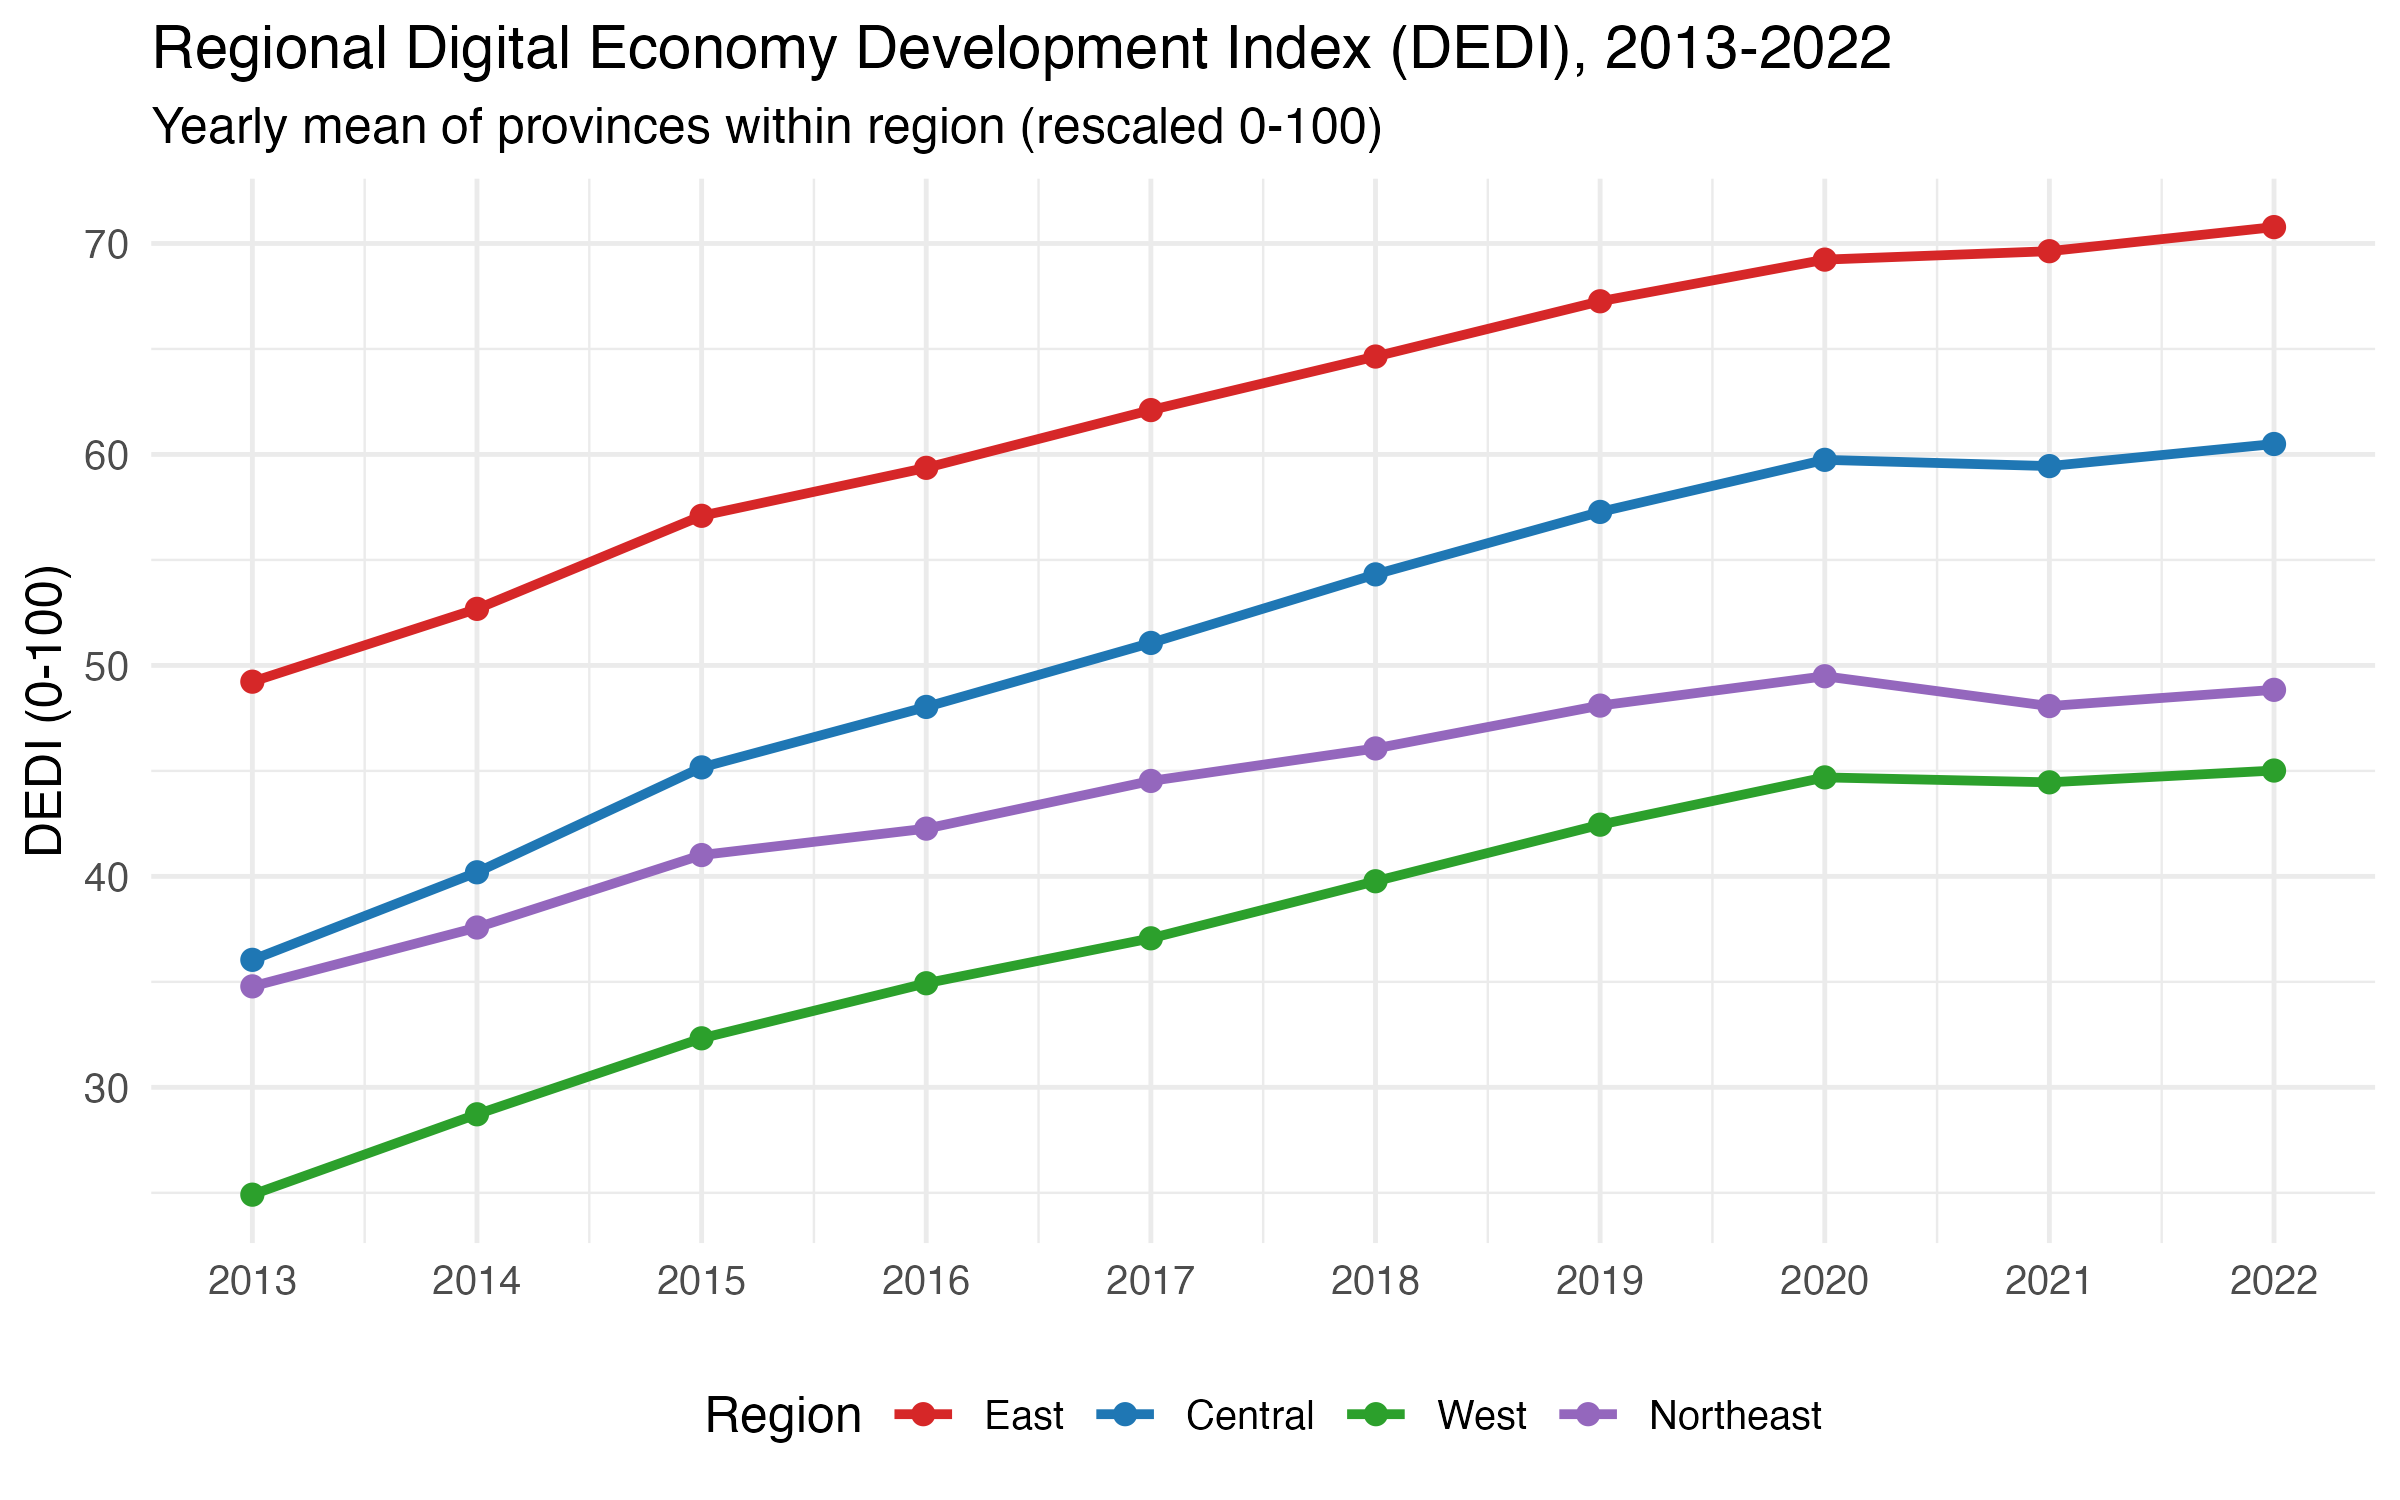
\includegraphics[width=\linewidth]{03_region_trend.png}
  \caption{Regional DEDI trajectories (yearly mean).}
\end{subfigure}\hfill
\begin{subfigure}[t]{0.49\textwidth}
  \centering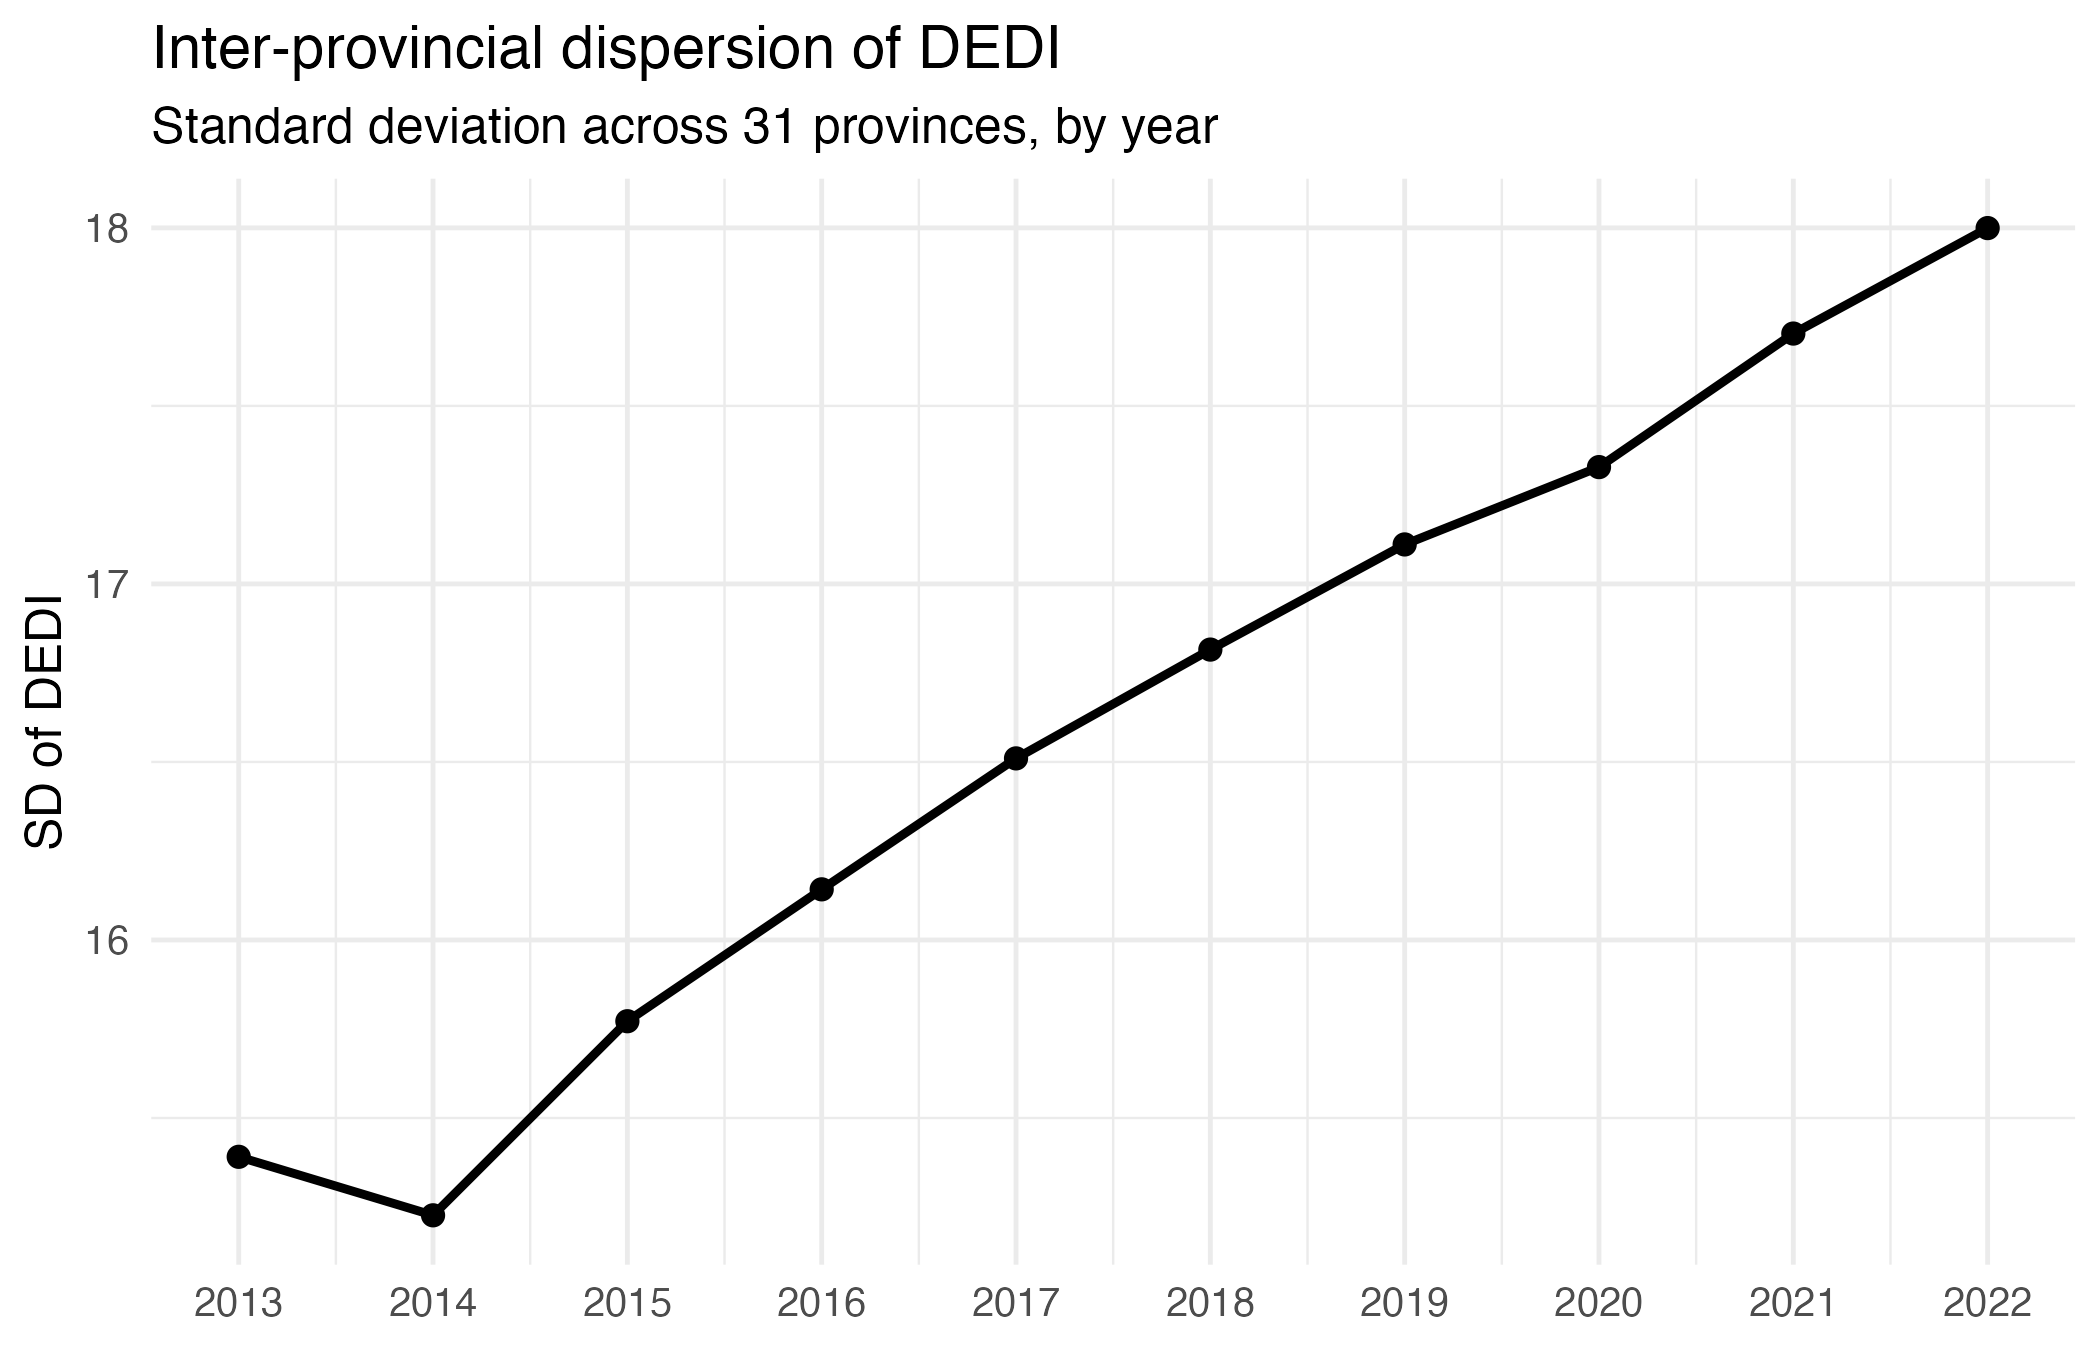
\includegraphics[width=\linewidth]{03_dispersion.png}
  \caption{Inter-provincial dispersion of DEDI.}
\end{subfigure}
\caption{DEDI temporal patterns, 2013--2022.}\label{fig:dedi-time}
\end{figure}

\subsection{MANOVA assumption diagnostics}

The four PC scores are mutually orthogonal by construction, so
multicollinearity --- the most consequential MANOVA assumption --- is
automatically satisfied.  Mardia's tests reject overall multivariate normality
(both skewness and kurtosis $p<.001$), but kurtosis holds within $8/8$
$\text{region}\times\text{period}$ cells while skewness holds within $4/8$
cells (Central, Northeast in both periods).  Box's $M$ rejects covariance
homogeneity across the eight cells, $\chi^{2}(70)=540.62$, $p<.001$, and
Levene's test rejects equal variances on PC1, PC2, and PC4.  Two multivariate
outliers are flagged at the $\chi^{2}_{.999,4}=18.47$ threshold (Tibet 2015,
2016).  Given these violations, Pillai's trace is adopted as the primary
multivariate criterion \citep{tabachnick2019}, and post hoc comparisons use
Welch's procedure with the Games--Howell adjustment \citep{games1976}.  Both
violations are revisited in Section~\ref{sec:sens} via robustness checks.

\subsection{Factorial MANOVA: main results}

Table~\ref{tab:manova} reports the omnibus tests.  Both main effects are
strongly significant under all four classical criteria, while the Region
$\times$ Period interaction is non-significant ($p=.892$, partial
$\eta^{2}=0.007$).  In substantive terms, every region advanced markedly
across the two periods, and they did so {in parallel}: the relative
rank-ordering of regions on the four-dimensional digital-economy construct
has not changed between 2013--2017 and 2018--2022.  The interaction plot
(Figure~\ref{fig:interaction}) makes the parallelism visually evident.



\begin{table}[H]
\centering
\caption{Factorial MANOVA: Region $\times$ Period (DVs $=$ PC1--PC4, $n=310$).}
\label{tab:manova}
\begin{tabular}{l r r l r r}
\toprule
\textbf{Effect} & \textbf{Pillai} $V$ & \textbf{$F$ (approx.)} & \textbf{$df_1, df_2$}
                & \textbf{$p$} & \textbf{Partial $\eta^{2}$}\\
\midrule
Region                  & 0.7537 &  25.25 & 12,\,903 & $<.001$ & $0.251$ \\
Period                  & 0.7188 & 191.12 &  4,\,299 & $<.001$ & $0.719$ \\
Region $\times$ Period  & 0.0213 &   0.54 & 12,\,903 & $.892$  & $0.007$ \\
\bottomrule
\end{tabular}
\end{table}

\begin{figure}[H]
\centering
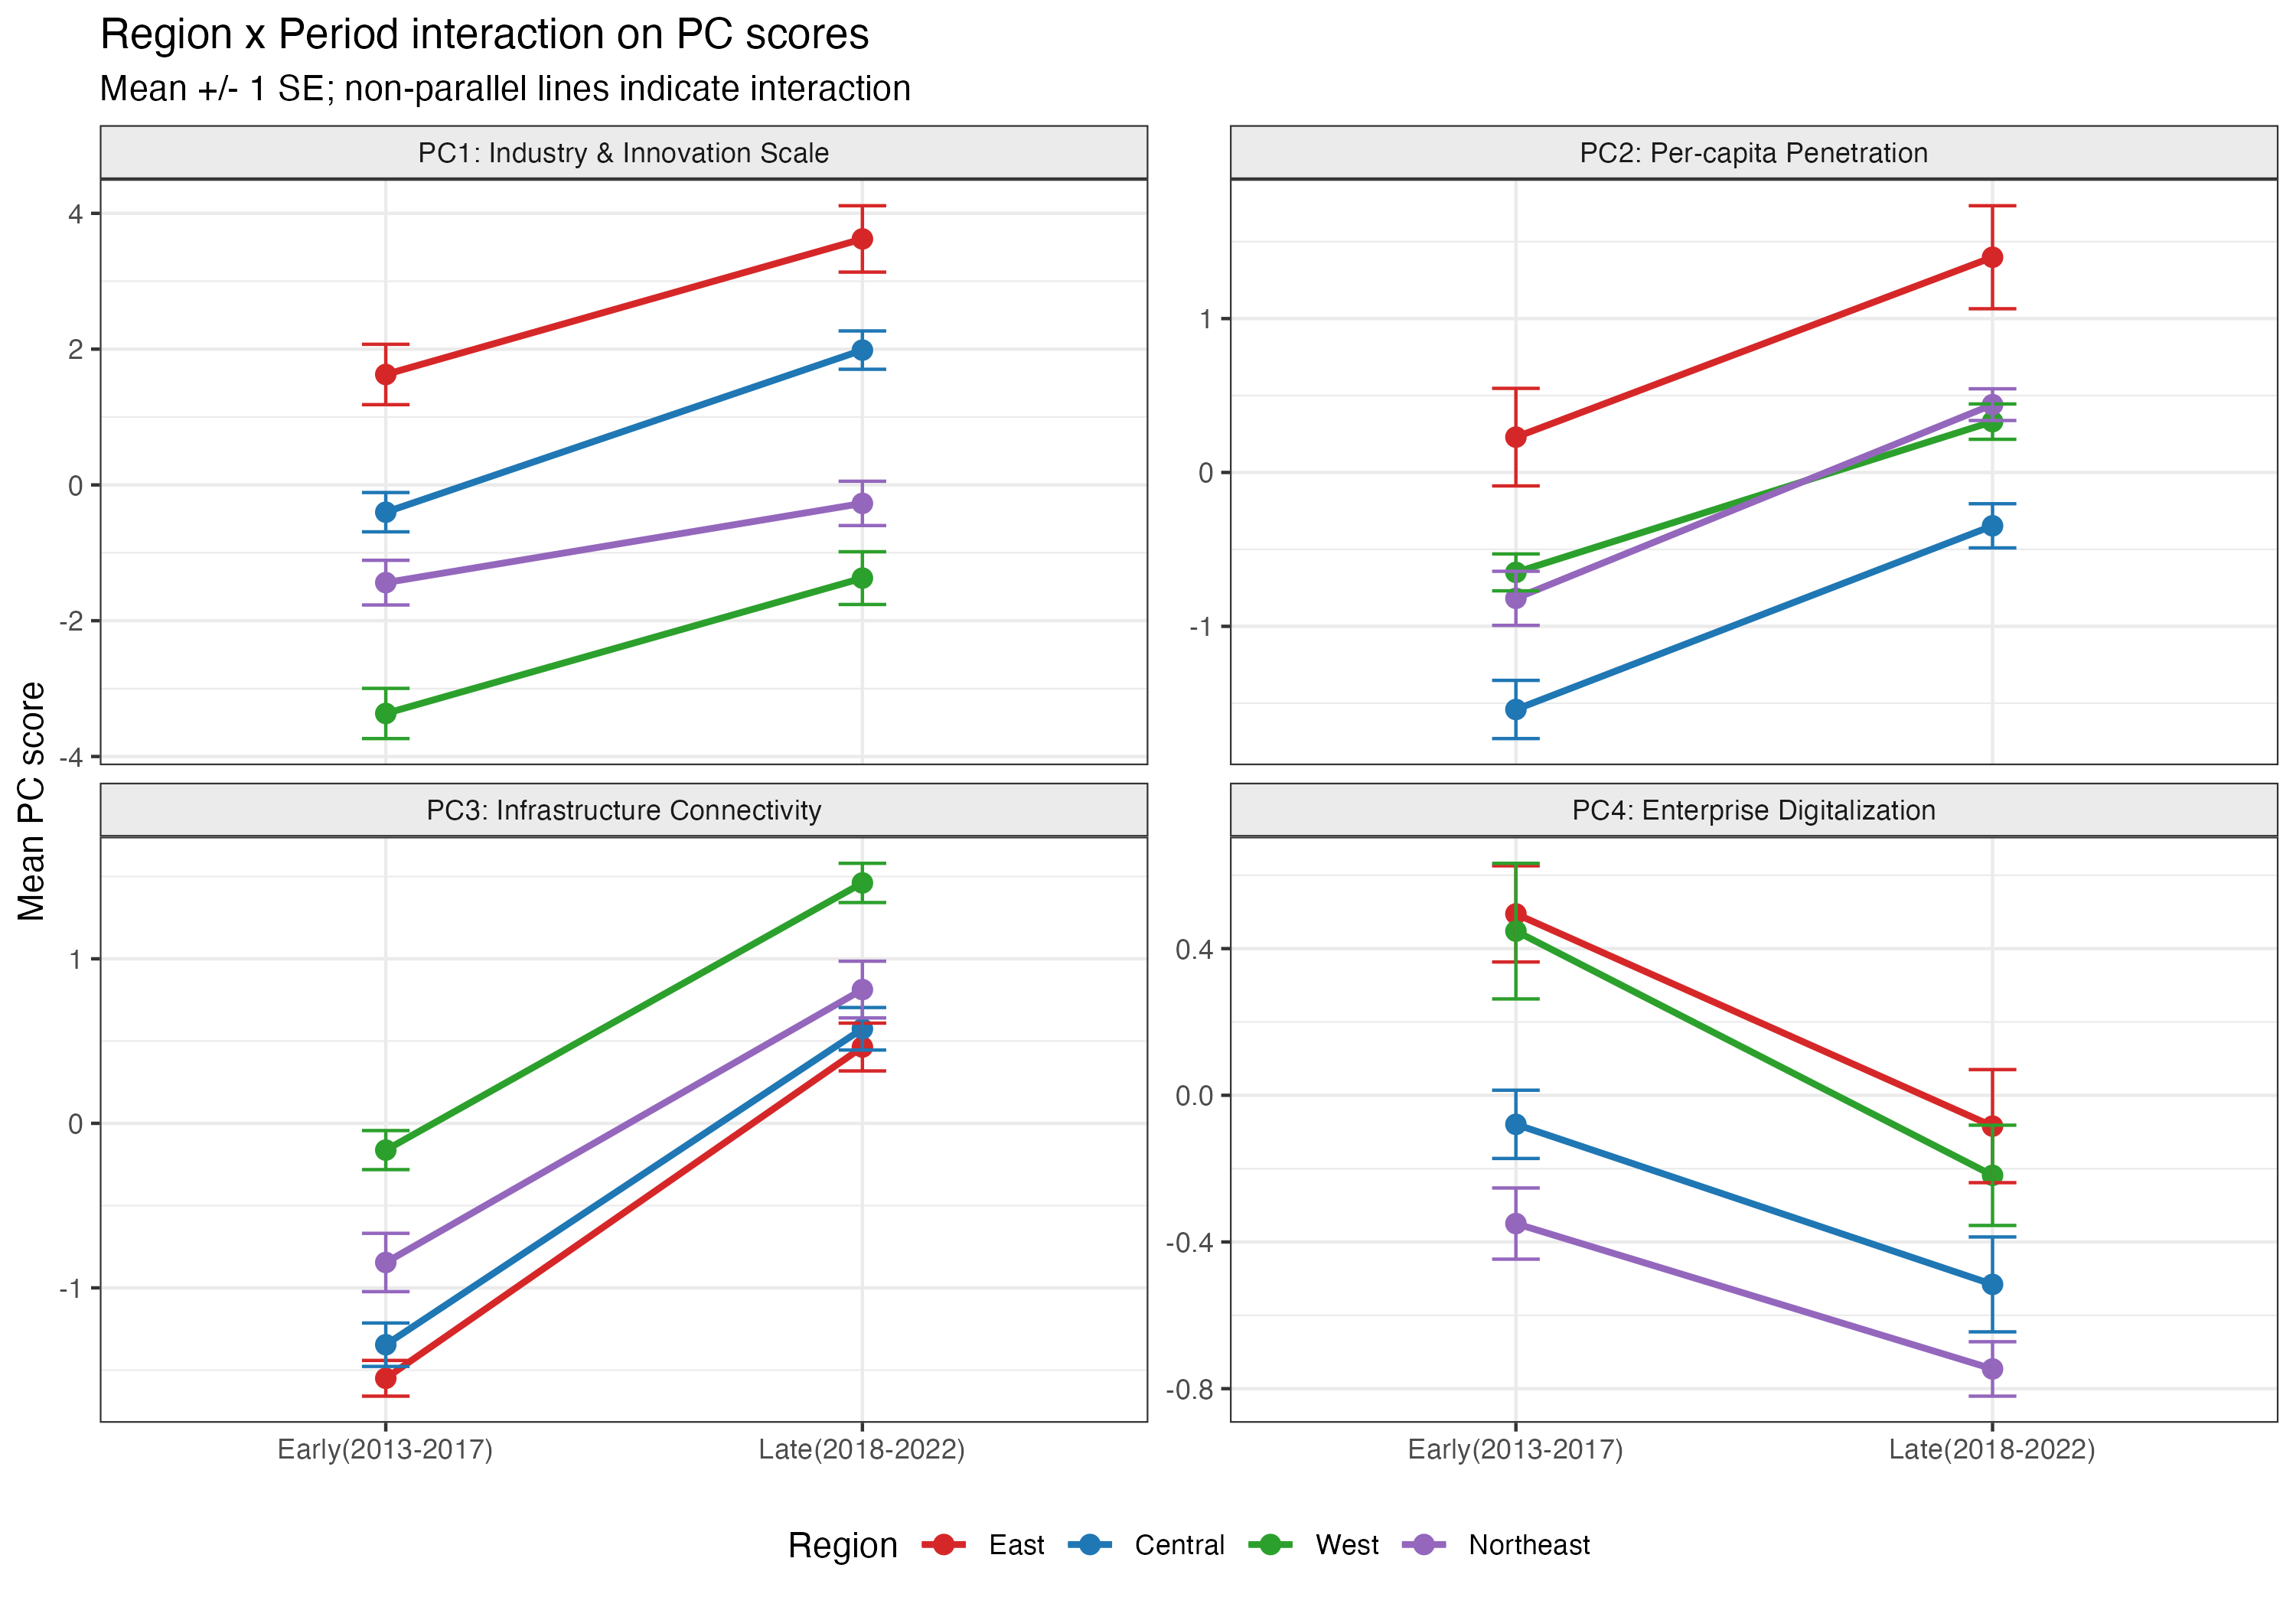
\includegraphics[width=0.95\textwidth]{05_interaction.png}
\caption{Region $\times$ Period interaction plot for the four PC scores.
Mean $\pm$ 1 SE within each cell.  Lines are nearly parallel, consistent with
the non-significant multivariate interaction reported in
Table~\ref{tab:manova}.}\label{fig:interaction}
\end{figure}

\subsection{Univariate decomposition and post hoc}

A univariate Type-II ANOVA decomposition shows that both main effects are
significant on each component (Table~\ref{tab:univ}).  Period is the dominant
source of variation on PC3 ({infrastructure}, $F = 343.6$,
$\eta^{2}_{p}=0.53$), reflecting a near-universal upgrading of broadband and
mobile networks during 2018--2022.  Region is the dominant source on PC1
({industry/innovation scale}, $F=63.0$).

\begin{table}[H]
\centering
\caption{Per-DV univariate ANOVA (Type II), $df_{\text{error}} = 302$.}
\label{tab:univ}
\small
\begin{tabular}{l r r r r r r}
\toprule
\textbf{Dependent variable} & \multicolumn{2}{c}{\textbf{Region}}
                            & \multicolumn{2}{c}{\textbf{Period}}
                            & \multicolumn{2}{c}{\textbf{Region $\times$ Period}}\\
            & $F(3,302)$ & $p$ & $F(1,302)$ & $p$ & $F(3,302)$ & $p$\\
\midrule
PC1 Industry / Innovation Scale   &  62.95 & $<.001$ &  40.78 & $<.001$ & 0.33 & $.80$\\
PC2 Per-capita Penetration        &  18.44 & $<.001$ &  42.60 & $<.001$ & 0.13 & $.94$\\
PC3 Infrastructure Connectivity   &  40.13 & $<.001$ & 343.62 & $<.001$ & 1.10 & $.35$\\
PC4 Enterprise Digitalization     &   6.47 & $<.001$ &  24.08 & $<.001$ & 0.25 & $.86$\\
\bottomrule
\end{tabular}
\end{table}

Games--Howell pairwise comparisons (collapsing across period) reveal that the
ordering of regions {varies by component}, exactly the kind of nuance that
a univariate analysis on a single composite would conceal.  On PC1
(industry/innovation scale) we find a strict ordering
$\text{East} > \text{Central} > \text{Northeast} > \text{West}$ with all six
pairs significant at $p<.001$.  On PC2 (per-capita penetration) the East
dominates, but the Central region is the {lowest} of the four ---
demonstrating that high industrial scale can coexist with relatively shallow
per-capita digital uptake.  On PC3 (infrastructure connectivity) only the West
is significantly below the other three regions, which are statistically
indistinguishable.  On PC4 (enterprise digitalization) the Northeast is the
lowest, with East $>$ Northeast significant at $p<.001$.

A complementary Welch period-contrast confirms that 2018--2022 means exceed
2013--2017 means on PC1 ($\Delta=1.99$, $p<.001$), PC2 ($\Delta=1.11$,
$p<.001$), and PC3 ($\Delta=1.81$, $p<.001$).  PC4 is the sole component to
{decline} between periods ($\Delta=-0.57$, $p<.001$): enterprise web
presence per $100$ firms peaked mid-decade and has been substituted by
mini-programs and platform super-apps.

\subsection{Sensitivity analyses}\label{sec:sens}

Three robustness checks support the main conclusions.

First, applying a one-way MANOVA on region to the single-year cross-sections
of 2018, 2019, and 2020 yields virtually identical Pillai statistics
($V = 0.897, 0.892, 0.893$) and consistently significant region effects
($p < .001$ in all three years).  The proposal's choice of 2019 as a benchmark
year is therefore not a special-case artefact.

Second, year-by-year PCAs run separately on 2013, 2018, and 2022 produce
loadings whose maximum absolute correlation with the full-panel loadings
exceeds $0.80$ for PC1, PC2, and PC4; PC3 (infrastructure) is the least stable
($r$ ranging from $0.33$ to $0.42$), reflecting the changing composition of
``infrastructure'' as broadband generations evolve.  This is acknowledged as a
limitation in the next section.

Third, refitting the factorial MANOVA after dropping the two outliers (Tibet
2015 and 2016) leaves the conclusions essentially unchanged: Pillai $V$ for
region is $0.754\to 0.754$, for period $0.719\to 0.717$, and for the interaction
$0.021\to 0.019$ (still non-significant).  The two outliers do not drive any
finding.

\begin{figure}[H]
\centering
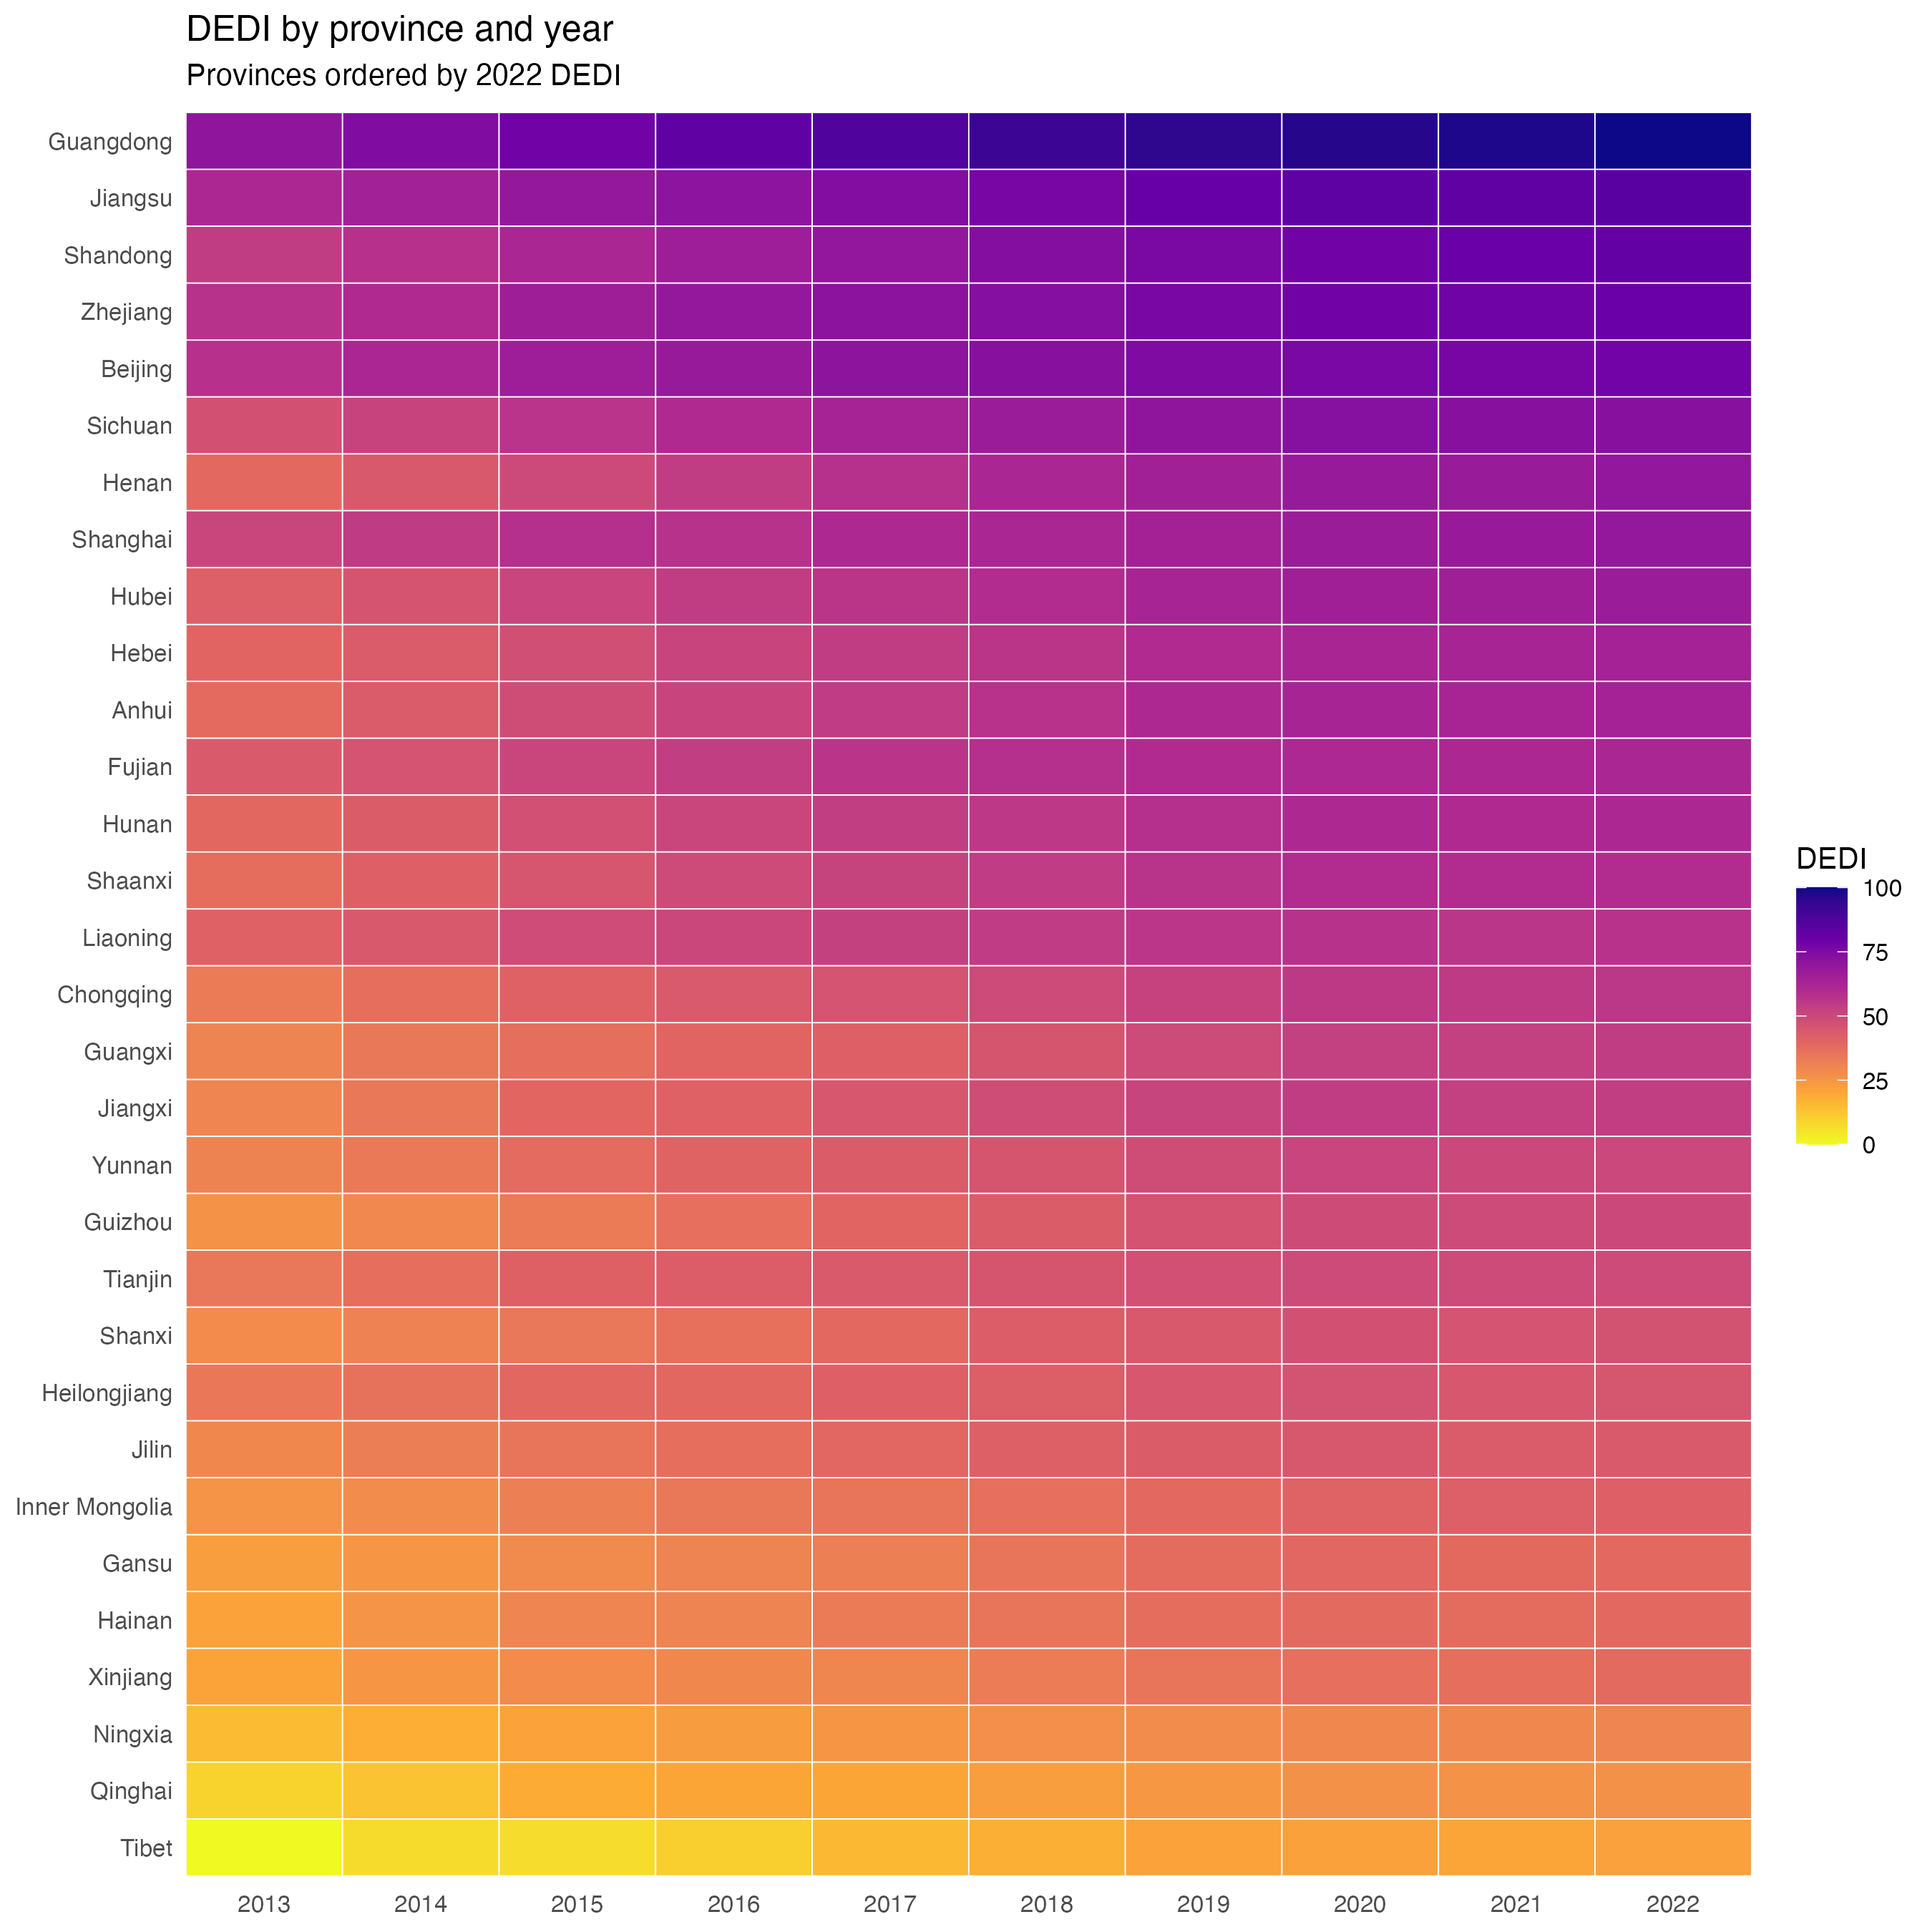
\includegraphics[width=0.85\textwidth]{03_dedi_heatmap.png}
\caption{DEDI by province and year, with provinces ordered by 2022 DEDI.
The diverging-magma palette highlights the persistent east--west gradient and
the rapid improvement of every province across the decade.}\label{fig:heatmap}
\end{figure}

% =========================================================================
\section{Discussion and Conclusion}\label{sec:discuss}
% =========================================================================

\subsection{Summary of findings}

Five conclusions emerge from the analysis.  {First}, four orthogonal
components --- industrial scale, per-capita penetration, infrastructure
connectivity, and enterprise digitalization --- adequately summarise the
22-indicator system, jointly explaining $85.8\%$ of variance.
{Second}, region is a large source of multivariate variation
($\eta^{2}=0.25$); the classic East-leads-West-lags gradient is statistically
robust.  {Third}, the period effect is even larger ($\eta^{2}=0.72$):
every region progressed markedly between the two five-year sub-periods on three
of the four components.  {Fourth}, the region-by-period interaction is
non-significant: regional gaps are shifting in absolute terms but {relative}
positions are essentially time-invariant.  {Fifth}, the multivariate
approach surfaces a nuance hidden by a single composite: the Central region
is high on industrial scale but low on per-capita penetration, while the
Northeast lags specifically on enterprise digitalization rather than
infrastructure.

\subsection{Theoretical and policy implications}

Methodologically, replacing hand-picked ``representative'' indicators with
orthogonal PC scores produces a clean, double-dipping-free MANOVA that
preserves all of the variance information of the original indicators.
Substantively, the absence of a Region $\times$ Period interaction implies
that the recent national push on broadband, 5G, and digital inclusive finance
has lifted all four regions, but has {not} re-shuffled the digital-economy
hierarchy.  Policymakers seeking spatial balance therefore cannot rely on
trickle-down from rising national averages; targeted interventions are needed
on the dimensions where specific regions lag.  In particular, the Central
region's relatively low per-capita penetration suggests scope for
consumer-facing diffusion programmes (digital training, e-commerce voucher
support), while the Northeast's enterprise-digitalization gap calls for
small-and-medium-enterprise digital-transformation subsidies similar to those
piloted in Zhejiang and Guangdong.

\subsection{Limitations}

Six limitations should temper interpretation.  (i)~The IPv4 indicator $x_5$
required imputation for $20.3\%$ of observations; while a re-run of the PCA
without $x_5$ leaves the loading structure of PC1, PC2, PC3 essentially
unchanged, the imputation introduces a degree of look-ahead bias.
(ii)~Multivariate normality is rejected by Mardia's tests even after
log-transformation; we mitigate by relying on the large-sample robustness of
Pillai's trace, but the 2019 cross-section ($n=31$) is more fragile.
(iii)~Box's $M$ is significant, indicating heteroscedasticity across regions;
Roy's largest-root statistic is reported alongside Pillai's $V$ for
transparency.  (iv)~The factorial design pools $310$ province--year observations
and does not explicitly model within-province autocorrelation; a province-level
random-effect or cluster-robust extension is left for future work.
(v)~The Northeast contributes only $30$ observations ($3$ provinces $\times 10$
years), giving low power for Northeast-specific contrasts.
(vi)~Two of the 22 indicators ($x_{16}$ digital inclusive finance index and
$x_{17}$ digital--real integration index) are themselves pre-aggregated
composite indices, raising a mild concern of double aggregation; nonetheless
their inclusion is consistent with mainstream Chinese digital-economy
measurement practice \citep{he2023,he2024}.

\subsection{Conclusion}

Combining principal component analysis with factorial MANOVA on the resulting
component scores, this study provides the first formal multivariate-inferential
evidence on the temporal stability of regional digital-economy disparities in
China.  We find that, while every region has progressed sharply between
2013--2017 and 2018--2022, the rank ordering of the four official economic
regions on a four-dimensional digital-economy construct has not changed.  The
substantive concern often voiced about the Northeast --- that it is being left
behind --- is real on the level dimension and on enterprise digitalization, but
not large enough to register as a multivariate interaction.  Future research
might extend this design to a Region $\times$ Period $\times$ Sector cube using
firm-level data, or use canonical correlation to relate the PC structure of
digital-economy supply to that of demand.

% =========================================================================
% Bibliography
% =========================================================================
\newpage
\addcontentsline{toc}{section}{References}

\begin{thebibliography}{99}
\setlength{\itemsep}{0.4em}\small

\bibitem[Bai et al.(2024)]{bai2024}
Bai, C., Lim, E. S., \& Chua, S. Y. (2024). A literature review of digital
economy measurement methods and indexes. {International Journal of Academic
Research in Business and Social Sciences}, 14(7), 1434--1450.
\href{https://doi.org/10.6007/IJARBSS/v14-i7/21740}{doi:10.6007/IJARBSS/v14-i7/21740}

\bibitem[Box(1949)]{box1949}
Box, G. E. P. (1949). A general distribution theory for a class of likelihood
criteria. {Biometrika}, 36(3--4), 317--346.

\bibitem[Games \& Howell(1976)]{games1976}
Games, P. A., \& Howell, J. F. (1976). Pairwise multiple comparison procedures
with unequal $n$'s and / or variances: A Monte Carlo study. {Journal of
Educational Statistics}, 1(2), 113--125.

\bibitem[He et al.(2023)]{he2023}
He, D., Zhao, X., \& Qi, Q. (2023). Measurement, spatial pattern and regional
difference of digital economy development in China. {Industrial Technology
\& Economy}, 42(3), 54--62. [In Chinese.]

\bibitem[He et al.(2024)]{he2024}
He, H., He, Z., \& Nie, X. (2024). Analysis and study of digital economy level
measurement index. {Journal of Internet and Digital Economics}, 4(3),
187--217.
\href{https://doi.org/10.1108/JIDE-05-2024-0020}{doi:10.1108/JIDE-05-2024-0020}

\bibitem[Kaiser(1974)]{kaiser1974}
Kaiser, H. F. (1974). An index of factorial simplicity. {Psychometrika},
39(1), 31--36.

\bibitem[Mardia(1970)]{mardia1970}
Mardia, K. V. (1970). Measures of multivariate skewness and kurtosis with
applications. {Biometrika}, 57(3), 519--530.

\bibitem[Pillai(1955)]{pillai1955}
Pillai, K. C. S. (1955). Some new test criteria in multivariate analysis.
{Annals of Mathematical Statistics}, 26(1), 117--121.

\bibitem[Tabachnick \& Fidell(2019)]{tabachnick2019}
Tabachnick, B. G., \& Fidell, L. S. (2019). {Using multivariate statistics}
(7th ed.). Pearson.

\end{thebibliography}

\end{document}
